\documentclass[12pt]{article}
\usepackage[margin=0.5in]{geometry}
\usepackage{hyperref,scrextend}
\setlength{\parindent}{0em}
\newcommand{\indentation}{2em}
\usepackage{mdframed}
\mdfdefinestyle{childframe}{%
	leftmargin=1em,%
	innerleftmargin=1em,%
	rightmargin=0,%
	innerrightmargin=0,%
	innertopmargin=0%,
	innerbottommargin=0%
	}

\newmdenv[%
  topline=false,%
  bottomline=false,%
  rightline=false,%
  skipabove=\topsep,%
  skipbelow=\topsep,%
  style=childframe,%
]{child}
\setcounter{secnumdepth}{0}
\usepackage{posets}
\begin{document}
\title{Posets\\\large v1.0.2.25.9.25.7.40.24}\author{William Gustafson}
\date{\today}
\maketitle
\tableofcontents
\setlength{\parskip}{\baselineskip}


{\list{}{\leftmargin 0.5cm}\item{
\section{Introduction}

This module provides a class \hyperlink{Poset}{\texttt{Poset}} that encodes a finite
partially ordered set (poset). Most notably, this module can efficiently
compute flag vectors, the \av\bv-index and the \cv\dv-index.
Quasigraded posets, in the sense of \cite{ehrenborg-goresky-readdy-15}, can be encoded and the \av\bv-index and \cv\dv-index of quasigraded
posets can be computed. Latex code
for Hasse diagrams can be produced with a very flexible interface.
There are
methods for common operations and constructions such as Cartesian products,
disjoint unions, interval lattices, lattice of ideals, etc. Various examples
of posets are provided such as Boolean algebras, the face lattice of the
$n$-dimensional cube, (noncrossing) partition lattices, the type $A_n$ Bruhat
and weak orders, uncrossing orders etc. General subposets can be
selected as well as particular ones of interest such as intervals and
rank selections. Posets from this
module can also be converted to and from posets from \href{https://www.sagemath.org}{sagemath} and \href{https://www.macaulay2.com/}{Macaulay2}.

Terminology and notation on posets generally follows \cite{stanley-12} and \cite{birkhoff-67}.

The full documentation for the current version can be \href{https://www.github.com/williamGustafson/posets/releases/latest/download/posets.pdf}{found here}.

\subsection{Installation}

Install with pip via \verb|python -m pip install posets|.
Alternatively, download the whl file \href{https://www.github.com/WilliamGustafson/posets/releases}{here} and install it with pip via \verb|python -m pip posets-*-py3-none-any.whl|.

\subsection{Usage}

Here we give an introduction to using the posets module.

In the code snippets below we assume the module is imported via

\verb|from posets import *|

Constructing a poset:
\begin{verbatim}P = Poset(relations={'':['a','b'],'a':['ab'],'b':['ab']})
Q = Poset(relations=[['','a','b'],['a','ab'],['b','ab']])
R = Poset(elements=['ab','a','b',''], less=lambda x,y: return x in y)
S = Poset(zeta = [[0,1,1,1],[0,0,0,1],[0,0,0,1],[0,0,0,0]], elements=['','a','b','ab'])
\end{verbatim}

Built in examples (see page~\pageref{Built in posets}):
\begin{verbatim}
Boolean(3) #Boolean algebra of rank 3
Cube(3) #Face lattice of the 3-dimensional cube
Bruhat(3) #Bruhat order on symmetric group of order 3!
Bnq(n=3,q=2) #Lattice of subspaces of F_2^3
DistributiveLattice(P) #lattice of ideals of P
Intervals(P) #meet semilattice of intervals of P
\end{verbatim}
These examples come with default drawing methods, for example,
when making latex code by calling \verb|DistributiveLattice(P).latex()|
the resulting figure depicts elements of the lattice as
Hasse diagrams of $P$ with elements of the ideal highlighted
(again, see page~\pageref{Built in posets}). Note, you will have
to set the \verb|height|, \verb|width| and possibly \verb|nodescale|
parameters in order to get sensible output.


Two posets compare equal when they have the same
set of elements and the same zeta values (i.e. the same order relation with the same weights):
\begin{verbatim}P == Q and Q == R and R == S #True
P == Poset(relations={'':['a','b']}) #False
P == Poset(relations={'':['ab'],'a':['ab'],'b':['ab']}) #False
P == Poset(zeta=[[0,1,1,2],[0,0,0,3],[0,0,0,4],[0,0,0,0]],
        elements=['','a','b','ab']) #False
\end{verbatim}

Use \hyperlink{Poset.is_isomorphic}{\texttt{is\_isomorphic}} or \hyperlink{PosetIsoClass}{\texttt{PosetIsoClass}} to check whether
posets are isomorphic:
\begin{verbatim}P.is_isomorphic(Boolean(2)) #True
P.isoClass()==Boolean(2).isoClass() #True
P.is_isomorphic(Poset(relations={'':['a','b']})) #False
\end{verbatim}

Viewing and creating Hasse diagrams:
\begin{verbatim}
P.show() #displays a Hasse diagram in a new window
P.latex() #returns latex code: \begin{tikzpicture}...
P.latex(standalone=True) #latex code for a
#standalone document: \documentclass{preview}...
display(P.img()) #Display a poset when in a Jupyter notebook
#this uses the output of latex()
\end{verbatim}

Computing invariants:
\begin{verbatim}
Cube(2).fVector() #{(): 1, (1,): 4, (2,): 4, (1, 2): 8}
Cube(2).hVector() #{(): 1, (1,): 3, (2,): 3, (1, 2): 1}
Boolean(5).sparseKVector() #{(3,): 8, (2,): 8, (1, 3): 4, (1,): 3, (): 1}
Boolean(5).cdIndex() #Polynomial({'ccd': 3, 'cdc': 5, 'dd': 4, 'dcc': 3, 'cccc': 1})
print(Boolean(5).cdIndex()) #c^{4}+3c^{2}d+5cdc+3dc^{2}+4d^{2}
\end{verbatim}

Polynomial operations:
\begin{verbatim}
#Create noncommutative polynomials from dictionaries,
#keys are monomials, values are coefficients
p=Polynomial({'ab':1})
q=Polynomial({'a':1,'b':1})

#get and set coefficients like a dictionary
q['a'] #1
q['x'] #0
p['ba'] = 1

#print latex
str(p) #ab+ba

#basic arithmetic, polynomials form an algebra
p+q #ab+ba+a+b
p*q #aba+ab^{2}+ba^{2}+bab
q*p #a^{2}b+aba+bab+b^{2}a
2*p #2ab+2ba
p**2 #abab+ab^{2}a+ba^{2}b+baba
p**(-1) #raises TypeError
p**q #raises TypeError

#substitutions and conversions
p.sub(q,'a') #ab+ba+2b^{2} substitute q for a in p
p.abToCd() #d rewrite a's and b's
#in terms of c=a+b and d=ab+ba when possible
Polynomial({'c':1,'d':1}).cdToAb() #a+b+ab+ba rewrite c's and d's
#in terms of a's and b's
\end{verbatim}

Converting posets to and from SageMath:
\begin{verbatim}
P.toSage() #Returns a SageMath class, must be run under sage
Poset.fromSage(Q) #Take a poset Q made with SageMath and return an instance of Poset
\end{verbatim}

Converting to and from Macaulay2:
\begin{verbatim}
-- In M2
load "convertPosets.m2" --Also loads Python and Posets packages
import "posets" --This module must be installed to system version of python
P = posets@@Boolean(3) --Calling python functions
pythonPosetToMac(P) --Returns an instance of the M2 class Posets
macPosetToPython(Q) --Take a poset made with M2 and return an
--instance of the python class Poset
\end{verbatim}

Quasigraded posets:
\begin{verbatim}
#Provide the zeta and rank functions explicitly
#To construct a 2-chain with top two elements rank 2 and 3
#and with zeta value -1 between minimum and the element covering it:
T = Poset([[1,-1,1],[1,1],[1]], ranks=[[0],[],[1],[2]])
\end{verbatim}
The poset \verb|T| above is from \cite[Example 6.14]{ehrenborg-goresky-readdy-15} with $M$ taken to
be the 3-dimensional solid torus.

You can calculate the flag vectors and the \cv\dv-index just as you would for a classical poset,
for example, \verb|T.cdIndex()| returns the polynomial $\cv^2-2\dv$.

When plotting a quasigraded poset by default only the underlying poset is shown with element heights
based on rank, the zeta values are not shown. If you wish to display the zeta values you can use
the class \hyperlink{ZetaHasseDiagram}{\texttt{ZetaHasseDiagram}} to draw a Hasse diagram of your poset with an element $p$ depicted as
the associated filter, namely the subposet $\{q:q\ge p\}$, and with elements of the filters labeled by the
corresponding zeta value. To do so, either construct the poset with \verb|hasse_class=ZetaHasseDiagram|
such as in \verb|Poset([[1,-1,1],[1,1],[1]], ranks=[[0],[],[1],[2]],hasse_class=ZetaHasseDiagram)| or
set the Hasse diagram attribute on the poset as below:
\begin{verbatim}
T = Poset([[1,-1,1],[1,1],[1]], ranks=[[0],[],[1],[2]])
T.hasseDiagram = ZetaHasseDiagram(T)
\end{verbatim}
You can also represent elements with ideals instead of filters by passing \verb|filters=False|.
See \hyperlink{ZetaHasseDiagram}{\texttt{ZetaHasseDiagram}} and \hyperlink{SubposetsHasseDiagram}{\texttt{SubposetsHasseDiagram}} for a thorough explanation of the options.

}\endlist}


\section{Poset}
\label{Poset}

\textbf{\hypertarget{Poset}{\Large \texttt{class Poset}}}

{\list{}{\leftmargin 0.5cm}\item{
A class representing a finite partially ordered set (possibly quasigraded).

Posets are encoded by a list \verb|elements|, a zeta
function \verb|zeta| describing the relations and a
list \verb|ranks| that specifies the length of each element.
Instances of \hyperlink{Poset}{\texttt{Poset}} also
have an attribute \verb|hasseDiagram| which is an instance
of the \hyperlink{HasseDiagram}{\texttt{HasseDiagram}} class used for plotting the poset.

To construct a poset you must pass one of the zeta matrix
matrix \verb|zeta|, a function \hyperlink{Poset.less}{\texttt{less}} or a list/dictionary
\hyperlink{Poset.relations}{\texttt{relations}} to describe
the relations. Additionally you may wish to specify the
elements as a list called \verb|elements| or by using
the \hyperlink{Poset.relations}{\texttt{relations}} argument. The full list of constructor
arguments are listed below.

Usually, the values of the zeta function are all 0 or 1,
with 1 indicating a relation. The given zeta function may
take other values, with 0 always indicating no relation
and any other value indicating a relation with the
specified weight. Additionally, if you provide a value
for \verb|ranks| you can specify any non-negative integer for
the ranks of elements.

\begin{itemize}
        \item[]{
        \verb|zeta| -- A triangular array indexed by $i,j$ such
        that $i<j$ whose entries are 0 if $i$ and $j$ are
        incomparable and otherwise an arbitrary weight. This
        argument may be an instance of \hyperlink{TriangularArray}{\texttt{TriangularArray}},
        a nested iterable or a flat iterable; in the latter case
        \verb|flat_zeta| should be \verb|True|. Elements are
        read row-wise when \verb|zeta| is an iterable.

        Note, unless \verb|trans_close| is \verb|False|
        it is only necessary to specify cover relations in the
        zeta matrix as the transitive closure will be computed.
        }
        \item[]{
        \verb|elements| -- A list specifying the elements of the poset.

                The default value is \verb|[0,...,len(zeta)-1]|
                Note, the list will be reordered into a linear extension as this is necessary to store the zeta function as a triangular array.
        }
        \item[]{
        \verb|ranks| -- A list of lists. The $i$th list is a list of indices of element of
                length $i$. This argument is inessential, if not provided it will be computed by the constructor.
                If constructing a large poset with an easily computed
                rank function you may wish to compute and pass the
                rank function to the constructor. This
                option is also useful if you are constructing
                a quasigraded poset, the provided rank list
                does not necessarily have to match up with
                the usual length function.
        }
        \item[]{
        \hyperlink{Poset.relations}{\texttt{relations}} -- Either a list of pairs $(x,y)$ such that $x<y$ or a dictionary
                whose values are lists of elements greater than the associated key.
                This is used to construct the zeta function if it is not provided.
                Note, it is only necessary to specify cover relations.
        }
        \item[]{
        \hyperlink{Poset.less}{\texttt{less}} -- A function that given two elements $p,q$ returns \verb|True| when
                $p < q$. This is used to construct the zeta function if neither \verb|zeta|
                nor \hyperlink{Poset.relations}{\texttt{relations}} are provided. It is only necessary to specify cover relations.
        }
        \item[]{
        \verb|indices| -- A boolean indicating indices instead of elements are used in
                \hyperlink{Poset.relations}{\texttt{relations}} and \hyperlink{Poset.less}{\texttt{less}}. The default is \verb|False|.
        }
        \item[]{
        \verb|name| -- An optional identifier. If not provided no name attribute is set.
        }
        \item[]{
        \verb|hasse_class| -- An instance of \verb|hasse_class| is constructed with arguments being
                this poset plus all keyword arguments passed to \hyperlink{Poset}{\texttt{Poset}}, i.e.:
                        \begin{verbatim}
                        this.hasseDiagram = hasse_class(this, **kwargs)
                        \end{verbatim}
                If you subclass \hyperlink{HasseDiagram}{\texttt{HasseDiagram}} to change default drawing behavior pass
                your subclass when constructing a poset.

                The default value is \hyperlink{HasseDiagram}{\texttt{HasseDiagram}}.
        }
        \item[]{
        \verb|trans_close| -- If \verb|True| the transitive closure of \verb|zeta| is
                computed, this should be \verb|False| only if the provided matrix satisfies
                \verb|zeta[i,j]==0| for $i$ and $j$ incomparable and \verb|zeta[i,j]!=0| otherwise.
                Similarly, if providing \hyperlink{Poset.relations}{\texttt{relations}} or \hyperlink{Poset.less}{\texttt{less}} the argument \verb|trans_close| should be \verb|False|
                only if all relations were specified by the
                given data.
        }
\end{itemize}
Any extra keyword arguments are passed to \hyperlink{HasseDiagram}{\texttt{HasseDiagram}} (or \verb|hasse_class|
if specified).


Function calls to several of the more costly computations are cached. Generally,
functions in this class do not change the poset but instead return a new poset.
\hyperlink{Poset}{\texttt{Poset}} objects may be considered immutable (this is not enforced in any way).
If you alter a poset you should clear the cache via: \verb|this.cache = {}|.



}\endlist}


\begin{child}
\subsection{Operations}
\label{Operations}

\textbf{\hypertarget{Poset.adjoin_onehat}{\texttt{def adjoin\_onehat(this, label=None)}}}
\addcontentsline{toc}{subsubsection}{\protect\hyperlink{Poset.adjoin_onehat}{adjoin\_onehat}}
{\list{}{\leftmargin 0.5cm}\item{
Returns a new poset with a new maximum adjoined.

The label default is the same as \hyperlink{Poset.adjoin_zerohat}{\texttt{Poset.adjoin\_zerohat}}


}\endlist}

\textbf{\hypertarget{Poset.adjoin_zerohat}{\texttt{def adjoin\_zerohat(this, label=None)}}}
\addcontentsline{toc}{subsubsection}{\protect\hyperlink{Poset.adjoin_zerohat}{adjoin\_zerohat}}
{\list{}{\leftmargin 0.5cm}\item{
Returns a new poset with a new minimum adjoined.

By default the label is the first non-negative integer that is not an element of the poset.


}\endlist}

\textbf{\hypertarget{Poset.bddProduct}{\texttt{def bddProduct(this, that)}}}
\addcontentsline{toc}{subsubsection}{\protect\hyperlink{Poset.bddProduct}{bddProduct}}
{\list{}{\leftmargin 0.5cm}\item{
Computes the Cartesian product of two posets with maximum and minimum adjoined, that is, the poset \[\big((P\wout\{\max P,\min P\})\times(Q\wout\{\max Q,\min Q\})\big)\cup\{\zerohat,\onehat\}.\]


}\endlist}

\textbf{\hypertarget{Poset.bddUnion}{\texttt{def bddUnion(this, that)}}}
\addcontentsline{toc}{subsubsection}{\protect\hyperlink{Poset.bddUnion}{bddUnion}}
{\list{}{\leftmargin 0.5cm}\item{
Computes the disjoint union of two posets with maximum and minimums identified, that is, the poset \[\big( (P\wout\{\max P,\min P\})\sqcup(Q\wout\{\max Q,\min Q\})\big)\cup\{\zerohat,\onehat\}.\]

The labels in the returned poset are the same as in \hyperlink{Poset.element_union}{\texttt{element\_union}}.


}\endlist}

\textbf{\hypertarget{Poset.cartesianProduct}{\texttt{def cartesianProduct(this, that)}}}
\addcontentsline{toc}{subsubsection}{\protect\hyperlink{Poset.cartesianProduct}{cartesianProduct}}
{\list{}{\leftmargin 0.5cm}\item{
Computes the Cartesian product.


}\endlist}

\textbf{\hypertarget{Poset.diamondProduct}{\texttt{def diamondProduct(this, that)}}}
\addcontentsline{toc}{subsubsection}{\protect\hyperlink{Poset.diamondProduct}{diamondProduct}}
{\list{}{\leftmargin 0.5cm}\item{
Computes the diamond product which is the Cartesian product of the two posets with their minimums removed and then adjoined with a new minimum.


}\endlist}

\textbf{\hypertarget{Poset.dual}{\texttt{def dual(this)}}}
\addcontentsline{toc}{subsubsection}{\protect\hyperlink{Poset.dual}{dual}}
{\list{}{\leftmargin 0.5cm}\item{
Returns the dual poset, this has the same elements and has relation $p\le q$ when $q\le p$ in the original poset.


}\endlist}

\textbf{\hypertarget{Poset.element_union}{\texttt{def element\_union(E, F)}}}
\addcontentsline{toc}{subsubsection}{\protect\hyperlink{Poset.element_union}{element\_union}}
{\list{}{\leftmargin 0.5cm}\item{
Computes the disjoint union of lists \verb|E| and \verb|F|.

If \verb|E| and \verb|F| have empty intersection return value is \verb|E+F|
otherwise return value is ($E\times\{0\})\cup(F\times\{1\}$). This is used by operation methods
such as \hyperlink{Poset.union}{\texttt{Poset.union}} and \hyperlink{Poset.starProduct}{\texttt{Poset.starProduct}}.


}\endlist}

\textbf{\hypertarget{Poset.identify}{\texttt{def identify(this, X, indices=False)}}}
\addcontentsline{toc}{subsubsection}{\protect\hyperlink{Poset.identify}{identify}}
{\list{}{\leftmargin 0.5cm}\item{
Returns a new poset after making identifications indicated by the argument \verb|X|.

The new relation is defined by $p\le q$ when there exists any representatives $p'$ and $q'$ such that $p'\le q'$ in the original poset.

The argument \verb|X| should either be a dictionary where keys are the representatives and the value is a list of elements
to identify with the key, or a list of lists where the first element of each list is the representative.
Trivial equivalence classes need not be specified.

Raises \verb|ValueError| if the identifications do not yield a poset (due to violation of the anti-symmetry axiom).


}\endlist}

\textbf{\hypertarget{Poset.prism}{\texttt{def prism(this)}}}
\addcontentsline{toc}{subsubsection}{\protect\hyperlink{Poset.prism}{prism}}
{\list{}{\leftmargin 0.5cm}\item{
Computes the prism of a poset, that is, the diamond product with \verb|Cube(1)|.


}\endlist}

\textbf{\hypertarget{Poset.pyr}{\texttt{def pyr(this)}}}
\addcontentsline{toc}{subsubsection}{\protect\hyperlink{Poset.pyr}{pyr}}
{\list{}{\leftmargin 0.5cm}\item{
Computes the pyramid of a poset, that is, the Cartesian product with a length 1 chain.


}\endlist}

\textbf{\hypertarget{Poset.starProduct}{\texttt{def starProduct(this, that)}}}
\addcontentsline{toc}{subsubsection}{\protect\hyperlink{Poset.starProduct}{starProduct}}
{\list{}{\leftmargin 0.5cm}\item{
Computes the star product of two posets.

This is the union of \verb|this| with the maximum removed and \verb|that| with the minimum
removed and all relations $p<q$ for $p$ in \verb|this| and $q$ in \verb|that|.


}\endlist}

\textbf{\hypertarget{Poset.union}{\texttt{def union(this, that)}}}
\addcontentsline{toc}{subsubsection}{\protect\hyperlink{Poset.union}{union}}
{\list{}{\leftmargin 0.5cm}\item{
Computes the disjoint union of two posets.

The labels in the returned poset are determined
by \hyperlink{Poset.element_union}{\texttt{element\_union}}.


}\endlist}

\subsection{Subposet Selection}
\label{Subposet Selection}

\textbf{\hypertarget{Poset.complSubposet}{\texttt{def complSubposet(this, S, indices=False)}}}
\addcontentsline{toc}{subsubsection}{\protect\hyperlink{Poset.complSubposet}{complSubposet}}
{\list{}{\leftmargin 0.5cm}\item{
Returns the subposet of elements not contained in \verb|S|.


}\endlist}

\textbf{\hypertarget{Poset.filter}{\texttt{def filter(this, x, indices=False, strict=False)}}}
\addcontentsline{toc}{subsubsection}{\protect\hyperlink{Poset.filter}{filter}}
{\list{}{\leftmargin 0.5cm}\item{
Returns the subposet of elements greater than or equal to any element of \verb|x|.

If \verb|strict| is \verb|True| then the element \verb|x| is not included in the returned poset and
if it is \verb|False| the element \verb|x| is included.

If \verb|indices| is \verb|True| then the element \verb|x| is interpreted as indices into the poset,
either way the return value is a subposet of the original poset.

Note, \verb|x| should not be an element of the poset but an iterable of elements; to construct a principal
filter for an element \verb|p| of a poset \verb|P| use \verb|P.filter((p,))|.


}\endlist}

\textbf{\hypertarget{Poset.ideal}{\texttt{def ideal(this, x, indices=False, strict=False)}}}
\addcontentsline{toc}{subsubsection}{\protect\hyperlink{Poset.ideal}{ideal}}
{\list{}{\leftmargin 0.5cm}\item{
Returns the subposet of elements less than or equal to any element of \verb|x|.

See \hyperlink{Poset.filter}{\texttt{Poset.filter}} for an explanation of the arguments.


}\endlist}

\textbf{\hypertarget{Poset.interval}{\texttt{def interval(this, i, j, indices=False)}}}
\addcontentsline{toc}{subsubsection}{\protect\hyperlink{Poset.interval}{interval}}
{\list{}{\leftmargin 0.5cm}\item{
Returns the closed interval $[i,j]$.


}\endlist}

\textbf{\hypertarget{Poset.max}{\texttt{def max(this, indices=False)}}}
\addcontentsline{toc}{subsubsection}{\protect\hyperlink{Poset.max}{max}}
{\list{}{\leftmargin 0.5cm}\item{
Returns a list of the maximal elements of the poset.


}\endlist}

\textbf{\hypertarget{Poset.min}{\texttt{def min(this, indices=False)}}}
\addcontentsline{toc}{subsubsection}{\protect\hyperlink{Poset.min}{min}}
{\list{}{\leftmargin 0.5cm}\item{
Returns a list of the minimal elements of the poset.


}\endlist}

\textbf{\hypertarget{Poset.properPart}{\texttt{def properPart(this)}}}
\addcontentsline{toc}{subsubsection}{\protect\hyperlink{Poset.properPart}{properPart}}
{\list{}{\leftmargin 0.5cm}\item{
Returns the subposet of all elements that are neither maximal nor minimal.


}\endlist}

\textbf{\hypertarget{Poset.rankSelection}{\texttt{def rankSelection(this, S)}}}
\addcontentsline{toc}{subsubsection}{\protect\hyperlink{Poset.rankSelection}{rankSelection}}
{\list{}{\leftmargin 0.5cm}\item{
Returns the subposet of elements whose rank is contained in \verb|S|.

Note, this does not automatically include the minimum or maximum.


}\endlist}

\textbf{\hypertarget{Poset.subposet}{\texttt{def subposet(this, S, indices=False, keep\_hasseDiagram=True)}}}
\addcontentsline{toc}{subsubsection}{\protect\hyperlink{Poset.subposet}{subposet}}
{\list{}{\leftmargin 0.5cm}\item{
Returns the subposet of elements in \verb|S|.


}\endlist}

\subsection{Internal Computations}
\label{Internal Computations}

\textbf{\hypertarget{Poset.isAntichain}{\texttt{def isAntichain(this, A, indices=False)}}}
\addcontentsline{toc}{subsubsection}{\protect\hyperlink{Poset.isAntichain}{isAntichain}}
{\list{}{\leftmargin 0.5cm}\item{
Returns whether the given set is an antichain ($i\not<j$ for all $i$ and $j$).


}\endlist}

\textbf{\hypertarget{Poset.join}{\texttt{def join(this, i, j, indices=False)}}}
\addcontentsline{toc}{subsubsection}{\protect\hyperlink{Poset.join}{join}}
{\list{}{\leftmargin 0.5cm}\item{
Computes the join of $i$ and $j$, if it does not exist returns \verb|None|.


}\endlist}

\textbf{\hypertarget{Poset.less}{\texttt{def less(this, i, j, indices=False)}}}
\addcontentsline{toc}{subsubsection}{\protect\hyperlink{Poset.less}{less}}
{\list{}{\leftmargin 0.5cm}\item{
Returns whether $i$ is strictly less than $j$.


}\endlist}

\textbf{\hypertarget{Poset.lesseq}{\texttt{def lesseq(this, i, j, indices=False)}}}
\addcontentsline{toc}{subsubsection}{\protect\hyperlink{Poset.lesseq}{lesseq}}
{\list{}{\leftmargin 0.5cm}\item{
Returns whether $i$ is less than or equal to $j$.


}\endlist}

\textbf{\hypertarget{Poset.mobius}{\texttt{def mobius(this, i=None, j=None, indices=False)}}}
\addcontentsline{toc}{subsubsection}{\protect\hyperlink{Poset.mobius}{mobius}}
{\list{}{\leftmargin 0.5cm}\item{
Computes the value of the M\"obius function from $i$ to $j$.

If neither $i$ nor $j$ are provided returns all values
of the M\"obius function as an instance of
\hyperlink{TriangularArray}{\texttt{TriangularArray}}.

If $i$ (respectively $j$) is not provided then it
is assumed to be the minimum (maximum) and raises 
an exception of type \verb|ValueError| if the poset
does not have a unique minimum (maximum).


}\endlist}

\textbf{\hypertarget{Poset.rank}{\texttt{def rank(this, i, indices=False)}}}
\addcontentsline{toc}{subsubsection}{\protect\hyperlink{Poset.rank}{rank}}
{\list{}{\leftmargin 0.5cm}\item{
Returns the length of $i$ (the length of the longest chain ending at $i$).

Returns \verb|None| if \verb|i| is not an element
(or \verb|i| is not a valid index if \verb|indices| is \verb|True|).


}\endlist}

\subsection{Queries}
\label{Queries}

\textbf{\hypertarget{Poset.covers}{\texttt{def covers(this, indices=False)}}}
\addcontentsline{toc}{subsubsection}{\protect\hyperlink{Poset.covers}{covers}}
{\list{}{\leftmargin 0.5cm}\item{
Returns the list of covers of the poset.

An element $q$ covers $p$ when $p<q$ and $p<r<q$ implies $r=p$ or $r=q$.


}\endlist}

\textbf{\hypertarget{Poset.isEulerian}{\texttt{def isEulerian(this)}}}
\addcontentsline{toc}{subsubsection}{\protect\hyperlink{Poset.isEulerian}{isEulerian}}
{\list{}{\leftmargin 0.5cm}\item{
Checks whether the given poset is Eulerian (every interval with at least 2 elements has an equal number of odd and even rank elements).


}\endlist}

\textbf{\hypertarget{Poset.isGorenstein}{\texttt{def isGorenstein(this)}}}
\addcontentsline{toc}{subsubsection}{\protect\hyperlink{Poset.isGorenstein}{isGorenstein}}
{\list{}{\leftmargin 0.5cm}\item{
Checks if the poset is Gorenstein*.

A poset is Gorenstein* if the proper part of all intervals with more than
two elements have sphere homology. In other words, this function checks that
\begin{center}
        \verb|this.interval(p,q).properPart().bettiNumbers()|
\end{center}
is either \verb|[2]| or \verb|[1,0,...,0,1]| for all $p\le q$ such that $\abs{\text{rk}(q)-\text{rk}(p)}\ge2$.


}\endlist}

\textbf{\hypertarget{Poset.isLattice}{\texttt{def isLattice(this)}}}
\addcontentsline{toc}{subsubsection}{\protect\hyperlink{Poset.isLattice}{isLattice}}
{\list{}{\leftmargin 0.5cm}\item{
Checks if the poset is a lattice.

Note, returns \verb|True| if \verb|this| is an empty poset.


}\endlist}

\textbf{\hypertarget{Poset.isRanked}{\texttt{def isRanked(this)}}}
\addcontentsline{toc}{subsubsection}{\protect\hyperlink{Poset.isRanked}{isRanked}}
{\list{}{\leftmargin 0.5cm}\item{
Checks whether the poset is ranked.


}\endlist}

\subsection{Invariants}
\label{Invariants}

\textbf{\hypertarget{Poset.abIndex}{\texttt{def abIndex(this)}}}
\addcontentsline{toc}{subsubsection}{\protect\hyperlink{Poset.abIndex}{abIndex}}
{\list{}{\leftmargin 0.5cm}\item{
Returns the \text{ab}-index of the poset as an instance of \hyperlink{Polynomial}{\texttt{Polynomial}}.

If the poset has a unique minimum and maximum but isn't ranked
this computes the \text{ab}-index considering the poset to be
quasigraded (in the sense of \cite{ehrenborg-goresky-readdy-15}) with $\overline{\zeta}=\zeta$ and $\rho$ the rank function $x\mapsto$\verb|P.rank(x)|. 

For more information on the \text{ab}-index see \cite{bayer-21}


}\endlist}

\textbf{\hypertarget{Poset.bettiNumbers}{\texttt{def bettiNumbers(this)}}}
\addcontentsline{toc}{subsubsection}{\protect\hyperlink{Poset.bettiNumbers}{bettiNumbers}}
{\list{}{\leftmargin 0.5cm}\item{
Computes the Betti numbers of the poset, that is, the ranks of the homology of the order complex (the simplicial complex of all chains).


}\endlist}

\textbf{\hypertarget{Poset.cdIndex}{\texttt{def cdIndex(this)}}}
\addcontentsline{toc}{subsubsection}{\protect\hyperlink{Poset.cdIndex}{cdIndex}}
{\list{}{\leftmargin 0.5cm}\item{
Returns the \textbf{cd}-index as an instance of \hyperlink{Polynomial}{\texttt{Polynomial}}.

If the given poset
does not have a \textbf{cd}-index then a \textbf{cd}-polynomial is still
returned, but this is not meaningful. If you wish to check whether a poset has
a \textbf{cd}-index then check the Boolean below:
\begin{center}
        \verb|this.abIndex().cdToAb()!=this.abIndex()|
\end{center}

If the given poset is semi-Eulerian then the \textbf{cd}-index
as defined in \cite{juhnke-kubitzke-24} is computed.

This function correctly computes the \cv\dv-index
of a quasigraded Eulerian poset (see \cite{ehrenborg-goresky-readdy-15}).

For computation we use the sparse $k$-vector formula see \cite[Proposition 7.1]{billera-ehrenborg-00}. For more info on the \textbf{cd}-index see \cite{bayer-21}.


}\endlist}

\textbf{\hypertarget{Poset.fVector}{\texttt{def fVector(this)}}}
\addcontentsline{toc}{subsubsection}{\protect\hyperlink{Poset.fVector}{fVector}}
{\list{}{\leftmargin 0.5cm}\item{
Returns flag $\overline{f}$-vector as a dictionary with keys $S\subseteq[n]$.

This method is intended for use with a poset, possibly quasi-graded, that has a unique minimum and maximum. On a classical poset this counts chains that contain the first
minimal element, \verb|this[this.ranks[0][0]]| and ignores the
final rank. 

Chains are weighted by the product of the zeta
values along the chain.


}\endlist}

\textbf{\hypertarget{Poset.flagVectors}{\texttt{def flagVectors(this)}}}
\addcontentsline{toc}{subsubsection}{\protect\hyperlink{Poset.flagVectors}{flagVectors}}
{\list{}{\leftmargin 0.5cm}\item{
Returns the table of flag $\overline{f}$- and $\overline{h}$-vectors as a dictionary with keys $S\subseteq[n]$ encoded as tuples and with elements \verb|(f_S, h_S)|.


}\endlist}

\textbf{\hypertarget{Poset.flagVectorsLatex}{\texttt{def flagVectorsLatex(this,standalone=False)}}}
\addcontentsline{toc}{subsubsection}{\protect\hyperlink{Poset.flagVectorsLatex}{flagVectorsLatex}}
{\list{}{\leftmargin 0.5cm}\item{
Returns a string of latex code representing the table of flag vectors of the poset.

Note, the package \href{https://ctan.org/pkg/longtable}{longtable} is required to compile the output.


}\endlist}

\textbf{\hypertarget{Poset.hVector}{\texttt{def hVector(this)}}}
\addcontentsline{toc}{subsubsection}{\protect\hyperlink{Poset.hVector}{hVector}}
{\list{}{\leftmargin 0.5cm}\item{
Returns the flag $\overline{h}$-vector of the poset.


}\endlist}

\textbf{\hypertarget{Poset.orderComplex}{\texttt{def orderComplex(this, indices=False)}}}
\addcontentsline{toc}{subsubsection}{\protect\hyperlink{Poset.orderComplex}{orderComplex}}
{\list{}{\leftmargin 0.5cm}\item{
Returns the poset of all chains ordered by inclusion.


}\endlist}

\textbf{\hypertarget{Poset.sparseKVector}{\texttt{def sparseKVector(this)}}}
\addcontentsline{toc}{subsubsection}{\protect\hyperlink{Poset.sparseKVector}{sparseKVector}}
{\list{}{\leftmargin 0.5cm}\item{
Returns the sparse $k$-vector $k_S = \sum_{T\subseteq S}(-1)^{\abs{S\wout T}}\overline{h}_T$.

The sparse $k$-vector only has entries $k_S$ for sparse sets $S$,
that is, sets $S\subseteq[\text{rk}(P)-1]$ such that if $i\in S$ then $i+1\not\in S$.
The sparse $k$-vector is returned as a dictionary whose keys are tuples.


}\endlist}

\subsection{Maps}
\label{Maps}

\textbf{\hypertarget{Poset.buildIsomorphism}{\texttt{def buildIsomorphism(this, that, indices=False)}}}
\addcontentsline{toc}{subsubsection}{\protect\hyperlink{Poset.buildIsomorphism}{buildIsomorphism}}
{\list{}{\leftmargin 0.5cm}\item{
Returns an isomorphism from \verb|this| to \verb|that| as a dictionary
or \verb|None| if the posets are not isomorphic.

If \verb|indices| is \verb|True| then the dictionary keys and values
are indices, otherwise they are elements.


}\endlist}

\textbf{\hypertarget{Poset.is_isomorphic}{\texttt{def is\_isomorphic(this, that)}}}
\addcontentsline{toc}{subsubsection}{\protect\hyperlink{Poset.is_isomorphic}{is\_isomorphic}}
{\list{}{\leftmargin 0.5cm}\item{
Returns \verb|True| if the posets are isomorphic and \verb|False| otherwise.


}\endlist}

\subsection{Miscellaneous}
\label{Miscellaneous}

\textbf{\hypertarget{Poset.__contains__}{\texttt{def \_\_contains\_\_(this, p)}}}
\addcontentsline{toc}{subsubsection}{\protect\hyperlink{Poset.__contains__}{\_\_contains\_\_}}
{\list{}{\leftmargin 0.5cm}\item{
Wrapper for \hyperlink{Poset.__contains__}{\texttt{this.elements.\_\_contains\_\_}}.


}\endlist}

\textbf{\hypertarget{Poset.__eq__}{\texttt{def \_\_eq\_\_(this,that)}}}
\addcontentsline{toc}{subsubsection}{\protect\hyperlink{Poset.__eq__}{\_\_eq\_\_}}
{\list{}{\leftmargin 0.5cm}\item{
Returns \verb|True| when \verb|that| is a \hyperlink{Poset}{\texttt{Poset}} representing the same poset as \verb|this| and \verb|False| otherwise.


}\endlist}

\textbf{\hypertarget{Poset.__getitem__}{\texttt{def \_\_getitem\_\_(this, i)}}}
\addcontentsline{toc}{subsubsection}{\protect\hyperlink{Poset.__getitem__}{\_\_getitem\_\_}}
{\list{}{\leftmargin 0.5cm}\item{
Wrapper for \hyperlink{Poset.__getitem__}{\texttt{this.elements.\_\_getitem\_\_}}.


}\endlist}

\textbf{\hypertarget{Poset.__hash__}{\texttt{def \_\_hash\_\_(this)}}}
\addcontentsline{toc}{subsubsection}{\protect\hyperlink{Poset.__hash__}{\_\_hash\_\_}}
{\list{}{\leftmargin 0.5cm}\item{
Hashes the poset, dependent on \verb|this.elements| and relations between
ranks.


}\endlist}

\textbf{\hypertarget{Poset.__init__}{\texttt{def \_\_init\_\_(this, zeta=None, elements=None, ranks=None, less=None, name='',}}}\\
\textbf{\texttt{hasse\_class=None, trans\_close=True, relations=None, indices=False, flat\_zeta=False, that=None,**kwargs)}}
\\
\addcontentsline{toc}{subsubsection}{\protect\hyperlink{Poset.__init__}{\_\_init\_\_}}
{\list{}{\leftmargin 0.5cm}\item{
See \hyperlink{Poset}{\texttt{Poset}}.


}\endlist}

\textbf{\hypertarget{Poset.__iter__}{\texttt{def \_\_iter\_\_(this)}}}
\addcontentsline{toc}{subsubsection}{\protect\hyperlink{Poset.__iter__}{\_\_iter\_\_}}
{\list{}{\leftmargin 0.5cm}\item{
Wrapper for \verb|this.elements__iter__|.


}\endlist}

\textbf{\hypertarget{Poset.__len__}{\texttt{def \_\_len\_\_(this)}}}
\addcontentsline{toc}{subsubsection}{\protect\hyperlink{Poset.__len__}{\_\_len\_\_}}
{\list{}{\leftmargin 0.5cm}\item{
Wrapper for \hyperlink{Poset.__len__}{\texttt{this.elements.\_\_len\_\_}}.


}\endlist}

\textbf{\hypertarget{Poset.__repr__}{\texttt{def \_\_repr\_\_(this)}}}
\addcontentsline{toc}{subsubsection}{\protect\hyperlink{Poset.__repr__}{\_\_repr\_\_}}
{\list{}{\leftmargin 0.5cm}\item{
Gives a string that can be evaluated to recreate the poset.

To use the returned string with \verb|eval| the claass \hyperlink{Poset}{\texttt{Poset}} must be in the namespace and \verb|repr(this.elements)|
must return a suitable string for evaluation.


}\endlist}

\textbf{\hypertarget{Poset.__str__}{\texttt{def \_\_str\_\_(this)}}}
\addcontentsline{toc}{subsubsection}{\protect\hyperlink{Poset.__str__}{\_\_str\_\_}}
{\list{}{\leftmargin 0.5cm}\item{
Returns a nicely formatted string listing the zeta matrix, the ranks list and the elements of the poset.


}\endlist}

\textbf{\hypertarget{Poset.chains}{\texttt{def chains(this, indices=False)}}}
\addcontentsline{toc}{subsubsection}{\protect\hyperlink{Poset.chains}{chains}}
{\list{}{\leftmargin 0.5cm}\item{
Returns a list of all nonempty chains of the poset (subsets $p_1<\dots<p_r$).


}\endlist}

\textbf{\hypertarget{Poset.copy}{\texttt{def copy(this)}}}
\addcontentsline{toc}{subsubsection}{\protect\hyperlink{Poset.copy}{copy}}
{\list{}{\leftmargin 0.5cm}\item{
Returns a shallow copy of the poset.

Making a shallow copy via the copy module i.e. \verb|Q = copy.copy(P)|
doesn't update the self reference in \verb|Q.hasseDiagram| (in this example
\verb|Q.hasseDiagram.P| is \verb|P|). This doesn't matter if you treat posets as immutable,
but otherwise could cause issues when displaying or generating hasse diagrams.
The returned poset has the self reference updated.


}\endlist}

\textbf{\hypertarget{Poset.fromSage}{\texttt{def fromSage(P)}}}
\addcontentsline{toc}{subsubsection}{\protect\hyperlink{Poset.fromSage}{fromSage}}
{\list{}{\leftmargin 0.5cm}\item{
Convert an instance of \verb|sage.combinat.posets.poset.FinitePoset| to an instance of \hyperlink{Poset}{\texttt{Poset}}.


}\endlist}

\textbf{\hypertarget{Poset.img}{\texttt{def img(this, tmpfile='a.tex', tmpdir=None, **kwargs)}}}
\addcontentsline{toc}{subsubsection}{\protect\hyperlink{Poset.img}{img}}
{\list{}{\leftmargin 0.5cm}\item{
Produces latex code (via calling \hyperlink{Poset.latex}{\texttt{latex}}) compiles it with pdflatex and returns a \verb|wand.image.Image| object constructed from the pdf.

In a Jupyter notebook calling \verb|display| on the return value will show the Hasse diagram in the output cell.
By default \verb|tmpdir| is \verb|tempfile.gettempdir()|.

This function converts the compiled pdf to an image using imagemagick, this may fail due to imagemagick's default security policies.
For more info and how to fix the issue see \url{https://askubuntu.com/questions/1127260/imagemagick-convert-not-allowed}

Keyword arguments are passed to \verb|latex()| but \verb|standalone| is alwasy set
to \verb|True| (otherwise the pdf would not compile).
Note this function may hang if \verb|pdflatex| fails
to compile.


}\endlist}

\textbf{\hypertarget{Poset.isoClass}{\texttt{def isoClass(this)}}}
\addcontentsline{toc}{subsubsection}{\protect\hyperlink{Poset.isoClass}{isoClass}}
{\list{}{\leftmargin 0.5cm}\item{
Returns an instance of \hyperlink{PosetIsoClass}{\texttt{PosetIsoClass}} representing the isomorphism class
of the poset.


}\endlist}

\textbf{\hypertarget{Poset.latex}{\texttt{def latex(this, **kwargs)}}}
\addcontentsline{toc}{subsubsection}{\protect\hyperlink{Poset.latex}{latex}}
{\list{}{\leftmargin 0.5cm}\item{
Returns a string of tikz code to draw the Hasse diagram of the poset for use in a \LaTeX{} document.

This is a wrapper for \hyperlink{Poset.latex}{\texttt{HasseDiagram.latex}}.

For a full list of keyword arguments see \hyperlink{HasseDiagram}{\texttt{HasseDiagram}}. The most common arguments are:
\begin{itemize}

        \item[]{\verb|height| -- The height in tikz units of the diagram.

                The default value is 10.
                }
        \item[]{\verb|width| -- The width in tikz units of the diagram.

                The default value is 8.
                }

        \item[]{\verb|labels| -- If \verb|False| elements are represented by filled circles.
                If \verb|True| by default elements are labeled by the result
                of casting the poset element to a string.

                The default value is \verb|True|.
                }

        \item[]{\verb|ptsize| -- When labels is \verb|False| this is the size of the circles used
                to represent elements. This has no effect if labels is \verb|True|.

                The default value is \verb|'2pt'|.
                }

        \item[]{\verb|nodescale| -- Each node is wrapped in \verb|'\\scalebox{'+nodescale+'}'|.

                The default value is \verb|'1'|.
                }

        \item[]{\verb|standalone| -- When \verb|True| a preamble is added to the beginning and
                \verb|'\\end{document}'| is added to the end so that the returned string
                is a full \LaTeX{} document that can be compiled. Compiling requires
                the \LaTeX{} packages tikz (pgf) and preview. The resulting figure can be
                incorporated into another \LaTeX{} document with \verb|\includegraphics|.

                When \verb|False| only the code for the figure is returned; the return value
                begins with \verb|\begin{tikzpicture}| and ends with \verb|\end{tikzpicture}|.

                The default is \verb|False|.
                }

        \item[]{\hyperlink{HasseDiagram.nodeLabel}{\texttt{nodeLabel}} -- A function that takes the \hyperlink{HasseDiagram}{\texttt{HasseDiagram}} object and an index
                and returns the label for the indicated element as a string.
                For example, the default implementation \hyperlink{HasseDiagram.nodeLabel}{\texttt{HasseDiagram.nodeLabel}}
                returns the element cast to a string and is defined as below:
                \begin{center}\begin{verbatim}
                        def nodeLabel(H, i):
                                return str(H.P[i])
                \end{verbatim}\end{center}

                Note \verb|H.P| is \verb|this|.
        }
\end{itemize}


}\endlist}

\textbf{\hypertarget{Poset.make_ranks}{\texttt{def make\_ranks(zeta)}}}
\addcontentsline{toc}{subsubsection}{\protect\hyperlink{Poset.make_ranks}{make\_ranks}}
{\list{}{\leftmargin 0.5cm}\item{
Used by the constructor to compute the ranks list for a poset when it isn't provided.


}\endlist}

\textbf{\hypertarget{Poset.relabel}{\texttt{def relabel(this, elements=None)}}}
\addcontentsline{toc}{subsubsection}{\protect\hyperlink{Poset.relabel}{relabel}}
{\list{}{\leftmargin 0.5cm}\item{
Returns a new \hyperlink{Poset}{\texttt{Poset}} object with
the \verb|elements| attribute as given.

If \verb|elements| is \verb|None| then
the returned poset has \verb|elements| attribute set to \verb|list(range(len(this)))|.


}\endlist}

\textbf{\hypertarget{Poset.relations}{\texttt{def relations(this, indices=False)}}}
\addcontentsline{toc}{subsubsection}{\protect\hyperlink{Poset.relations}{relations}}
{\list{}{\leftmargin 0.5cm}\item{
Returns a list of all pairs $(e,f)$ where $e\le f$.


}\endlist}

\textbf{\hypertarget{Poset.reorder}{\texttt{def reorder(this, perm, indices=False)}}}
\addcontentsline{toc}{subsubsection}{\protect\hyperlink{Poset.reorder}{reorder}}
{\list{}{\leftmargin 0.5cm}\item{
Returns a new \hyperlink{Poset}{\texttt{Poset}} object (representing the same poset) with the elements reordered.

\verb|perm| should be a list of elements if \verb|indices| is \verb|False| or a list of indices if \verb|True|.
The returned poset has elements in order of a linear
extension created from the given permutation.
If the list \verb|perm| defines a linear
extension then \verb|perm[i]| is the $i$th element.

If \verb|perm| is not a linear extension it is coerced into a
linear extension by repeatedly removing the first
element whose ideal has already been removed.


}\endlist}

\textbf{\hypertarget{Poset.show}{\texttt{def show(this, **kwargs)}}}
\addcontentsline{toc}{subsubsection}{\protect\hyperlink{Poset.show}{show}}
{\list{}{\leftmargin 0.5cm}\item{
Opens a window displaying the Hasse diagram of the poset.

This is a wrapper for \hyperlink{HasseDiagram.tkinter}{\texttt{HasseDiagram.tkinter}}.

For a full list of keyword arguments see \hyperlink{HasseDiagram}{\texttt{HasseDiagram}}. The most common arguments are:
\begin{itemize}
        \item[]{\verb|height| -- The height of the diagram.

                The default value is 10.
        }

        \item[]{\verb|width| -- The width of the diagram.

                The default width is 8.
        }

        \item[]{\verb|labels| -- If \verb|False| elements are represented as filled circles.
                If \verb|True| by default elements are labeled by the result of
                casting the poset element to a string.

                The default value is \verb|True|.
        }

        \item[]{\verb|ptsize| -- When labels is \verb|False| controls the size of the circles
                representing elements. This can be an integer or a string,
                if the value is a string the last two characters are ignored.

                The default value is \verb|'2pt'|.
        }

        \item[]{\verb|scale| -- Scale of the diagram.

                The default value is 1.
        }

        \item[]{\verb|padding| -- A border of this width is added around all sides of the diagram.

                The default value is 1.
        }

        \item[]{\hyperlink{HasseDiagram.nodeLabel}{\texttt{nodeLabel}} -- A function that takes the \hyperlink{HasseDiagram}{\texttt{HasseDiagram}} object and an index
                and returns the label for the indicated element as a string.
                For example, the default implementation \hyperlink{HasseDiagram.nodeLabel}{\texttt{HasseDiagram.nodeLabel}}
                returns the element cast to a string and is defined as below:
                \begin{center}\begin{verbatim}
                        def nodeLabel(H, i):
                                return str(H.P[i])
                \end{verbatim}\end{center}
                Note \verb|H.P| is \verb|this|.
        }
\end{itemize}


}\endlist}

\textbf{\hypertarget{Poset.shuffle}{\texttt{def shuffle(this)}}}
\addcontentsline{toc}{subsubsection}{\protect\hyperlink{Poset.shuffle}{shuffle}}
{\list{}{\leftmargin 0.5cm}\item{
Returns a new \hyperlink{Poset}{\texttt{Poset}} object (representing the same poset) with the elements in a random order.


}\endlist}

\textbf{\hypertarget{Poset.sort}{\texttt{def sort(this, key = None, indices=False)}}}
\addcontentsline{toc}{subsubsection}{\protect\hyperlink{Poset.sort}{sort}}
{\list{}{\leftmargin 0.5cm}\item{
Returns a new \hyperlink{Poset}{\texttt{Poset}} object (representing the same poset) with the elements sorted.

If the given key does not deifine a linear
extension then the ordering is coerced
to one in the same way as \hyperlink{Poset.reorder}{\texttt{reorder}}.


}\endlist}

\textbf{\hypertarget{Poset.toSage}{\texttt{def toSage(this)}}}
\addcontentsline{toc}{subsubsection}{\protect\hyperlink{Poset.toSage}{toSage}}
{\list{}{\leftmargin 0.5cm}\item{
Converts the poset to an instance of \verb|sage.combinat.posets.posets.FinitePoset|.


}\endlist}

\textbf{\hypertarget{Poset.transClose}{\texttt{def transClose(T)}}}
\addcontentsline{toc}{subsubsection}{\protect\hyperlink{Poset.transClose}{transClose}}
{\list{}{\leftmargin 0.5cm}\item{
Given an instance of \hyperlink{TriangularArray}{\texttt{TriangularArray}} encoding a (possibly weighted) relation, via $x\sim y$ when the $x,y$ entry is nonzero computes the transitive closure.

Note, an induced relation $i<j$ is weighted
by \verb|T[i,k]*T[k,j]| where $j$ and $k$ are
the minimal indices greater than $i$ satisfying
the conditions \verb|T[i,k]!=0| and \verb|T[k,j]!=0|.


}\endlist}

\textbf{\hypertarget{Poset.zeta_from_relations}{\texttt{def zeta\_from\_relations(relations,elements)}}}
\addcontentsline{toc}{subsubsection}{\protect\hyperlink{Poset.zeta_from_relations}{zeta\_from\_relations}}
{\list{}{\leftmargin 0.5cm}\item{
Given a dictionary of relations and a list of elements returns the zeta matrix and the elements reordered in a linear extension.

The dictionary \hyperlink{Poset.relations}{\texttt{relations}} should have keys that are indices into the list \verb|elements| and values that are lists of indices 
into \verb|elements|. If an index \verb|i| is contained in the list \verb|relations[j]| then  the $j$th elements is
less than the $i$th element in the poset.


}\endlist}

\textbf{\hypertarget{Poset.linearize}{\texttt{def linearize(this, X, indices=False)}}}
\addcontentsline{toc}{subsection}{\protect\hyperlink{Poset.linearize}{linearize}}
{\list{}{\leftmargin 0.5cm}\item{
Given a list \verb|X| of elements, returns a new list of the elements in a linear extension of the subposet.
}\endlist}

\end{child}



\section{PosetIsoClass}
\label{PosetIsoClass}

\textbf{\hypertarget{PosetIsoClass}{\Large \texttt{class PosetIsoClass(Poset)}}}

{\list{}{\leftmargin 0.5cm}\item{
This class encodes the isomorphism type of a poset.

Internally, this class inherits from \hyperlink{Poset}{\texttt{Poset}} and thus instances of
\hyperlink{PosetIsoClass}{\texttt{PosetIsoClass}} are also instances of \hyperlink{Poset}{\texttt{Poset}}.
The major differences between this class
and \hyperlink{Poset}{\texttt{Poset}} are that \verb|PosetIsoClass.__eq__| returns \verb|True|
when the two posets are isomorphic and all methods in \hyperlink{Poset}{\texttt{Poset}}
that return a \hyperlink{Poset}{\texttt{Poset}} object in \hyperlink{PosetIsoClass}{\texttt{PosetIsoClass}} instead return
an instance of \hyperlink{PosetIsoClass}{\texttt{PosetIsoClass}}.

Construct an instance of \hyperlink{PosetIsoClass}{\texttt{PosetIsoClass}} the same way as you would an
instance of \hyperlink{Poset}{\texttt{Poset}} or given a poset \verb|P| use \verb|P.isoClass()|.


}\endlist}

\section{Genlatt}
\label{Genlatt}

\textbf{\hypertarget{Genlatt}{\Large \texttt{class Genlatt(Poset)}}}

{\list{}{\leftmargin 0.5cm}\item{
A class to encode a ``generator-enriched lattice'' which is a lattice $L$
along with a set $G\subseteq L\wout\{\zerohat\}$ that generates $L$
under the join operation.

This class is mainly provided for the \hyperlink{Genlatt.minorPoset}{\texttt{minorPoset}} method.

Constructor arguments are the same as for \hyperlink{Poset}{\texttt{Poset}} except that
this constructor accepts two additional keyword only arguments:
        \begin{itemize}
                \item{\verb|G| - An iterable specifying the
                        generating set, can either contain
                        elements of the lattice or indices into
                        the lattice. The join irreducibles are automatically
                        added and may be omitted. If \verb|G| is not
                        provided the generating set will consist of the
                        join irreducibles.}
                \item{\verb|G_indices| - If \verb|True| then the provided
                        argument \verb|G| should
                        consist of indices otherwise \verb|G| should
                        consist of elements.}
        \end{itemize}

Note, a lattice $L$ enriched with a generating set $G$ is denoted
as the pair $(L,G)$.
See \cite{gustafson-23} for more on {generator-enriched lattices}\footnote{perhaps too much more}.


}\endlist}


\begin{child}
\textbf{\hypertarget{Genlatt.Del}{\texttt{def Del(this, K)}}}
\addcontentsline{toc}{subsection}{\protect\hyperlink{Genlatt.Del}{Del}}
{\list{}{\leftmargin 0.5cm}\item{
Return the deletion set of the minor \verb|K|.

The argument \verb|K| should be an instance of \hyperlink{Genlatt}{\texttt{Genlatt}}.

The deletion set of a minor $(K,H)$ of $(L,G)$ is the set
\[\text{Del}(K,H)=\{g\in G:g\join\zerohat_K\not\in H\cup\{\zerohat_K\}\}\]
This is the minimal set of generators that must be deleted
to form $(K,H)$ from $(L,G)$.
}\endlist}

\textbf{\hypertarget{Genlatt.__init__}{\texttt{def \_\_init\_\_(this, *args, G=None, G\_indices=False, **kwargs)}}}
\addcontentsline{toc}{subsection}{\protect\hyperlink{Genlatt.__init__}{\_\_init\_\_}}
{\list{}{\leftmargin 0.5cm}\item{
See \hyperlink{Genlatt}{\texttt{Genlatt}}.
}\endlist}

\textbf{\hypertarget{Genlatt._minors}{\texttt{def \_minors(this, minors, rels, i, weak, L)}}}
\addcontentsline{toc}{subsection}{\protect\hyperlink{Genlatt._minors}{\_minors}}
{\list{}{\leftmargin 0.5cm}\item{
Recursion backend to \hyperlink{Genlatt.minors}{\texttt{minors}}.
}\endlist}

\textbf{\hypertarget{Genlatt.contract}{\texttt{def contract(this, g, weak=False, L=None)}}}
\addcontentsline{toc}{subsection}{\protect\hyperlink{Genlatt.contract}{contract}}
{\list{}{\leftmargin 0.5cm}\item{
Return the \hyperlink{Genlatt}{\texttt{Genlatt}} obtained by contracting the generator \verb|g|, if \verb|weak| is \verb|True| performs the weak contraction with respect to \verb|L| (default value for \verb|L| is \verb|this|).
}\endlist}

\textbf{\hypertarget{Genlatt.delete}{\texttt{def delete(this, g)}}}
\addcontentsline{toc}{subsection}{\protect\hyperlink{Genlatt.delete}{delete}}
{\list{}{\leftmargin 0.5cm}\item{
Return the \hyperlink{Genlatt}{\texttt{Genlatt}} obtained by deleting the generator \verb|g|.
}\endlist}

\textbf{\hypertarget{Genlatt.minor}{\texttt{def minor(this, H, z)}}}
\addcontentsline{toc}{subsection}{\protect\hyperlink{Genlatt.minor}{minor}}
{\list{}{\leftmargin 0.5cm}\item{
Given an iterable \verb|H| of generators and an element \verb|z| returns the \hyperlink{Genlatt}{\texttt{Genlatt}} with minimum \verb|z| and generating
set \verb|H| and with the same order as \verb|this|.
}\endlist}

\textbf{\hypertarget{Genlatt.minorPoset}{\texttt{def minorPoset(this, weak=False, **kwargs)}}}
\addcontentsline{toc}{subsection}{\protect\hyperlink{Genlatt.minorPoset}{minorPoset}}
{\list{}{\leftmargin 0.5cm}\item{
        Returns the minor poset of the given \hyperlink{Genlatt}{\texttt{Genlatt}} instance.

        When generating a Hasse diagram with \verb|latex()| use
the prefix \verb|L_| to control options for the node diagrams.
        }\endlist}

\textbf{\hypertarget{Genlatt.minors}{\texttt{def minors(this, weak=False)}}}
\addcontentsline{toc}{subsection}{\protect\hyperlink{Genlatt.minors}{minors}}
{\list{}{\leftmargin 0.5cm}\item{
Returns a list of minors of the given \hyperlink{Genlatt}{\texttt{Genlatt}} instance
and an incomplete dictionary of relations.

The relations when transitively closed yield the relations
for the minor poset.
}\endlist}

\end{child}



\section{HasseDiagram}
\label{HasseDiagram}

\textbf{\hypertarget{HasseDiagram}{\Large \texttt{class HasseDiagram}}}

{\list{}{\leftmargin 0.5cm}\item{
A class that can produce latex/tikz code for the Hasse diagram of a poset or display the diagram in a window using tkinter.


\textbf{\large{Overview}}

An instance of this class is attached to each instance of \hyperlink{Poset}{\texttt{Poset}}. This class
is used to produce latex code for a poset when \verb|Poset.latex()| is called or
to display a poset in a new window when \verb|Poset.show()| is called. These functions
are wrappers for \verb|HasseDiagram.latex()| and \verb|HasseDiagram.tkinter()|.

The constructor for this class takes keyword arguments that control how the
Hasse diagram is drawn. These keyword arguments set the default options
for that given instance of \hyperlink{HasseDiagram}{\texttt{HasseDiagram}}. When calling \verb|latex()|
to produce latex code
or \verb|tkinter()| to draw the diagram in a tkinter window the same keyword arguments can
be passed to control how the diagram is drawn during that particular operation.

There are two types of options: constant values such as
\verb|height|,\verb|width| or \verb|scale| and function
values such as \hyperlink{HasseDiagram.loc_x}{\texttt{loc\_x}}, \hyperlink{HasseDiagram.loc_y}{\texttt{loc\_y}} or \hyperlink{HasseDiagram.nodeLabel}{\texttt{nodeLabel}}.

\textbf{\large Keyword arguments}

Options that affect both \verb|latex()| and \verb|tkinter()|:

        \begin{itemize}

        \item[]{\verb|width| -- Width of the diagram. When calling \verb|latex()| this is the width
                in tikz units (by default centimeters), for \verb|tkinter()| the units are $\frac{1}{30}$th of tkinter's units.

                The default value is 8.
        }

        \item[]{\verb|height| -- Height of the diagram, uses the same units as width.

                The default value is 10.
        }

        \item[]{\verb|labels| -- If this is \verb|True| display labels, obtained from \verb|nodeLabels|, for elements; if this is \verb|False| display filled circles for elements.
                The default value is \verb|True|.
        }

        \item[]{\verb|ptsize| -- No effect when \verb|labels| is \verb|True|, when \verb|labels| is \verb|False| this is the size
                of the circles shown for elements. When calling \verb|tkinter()| this can
                be either a number or a string. For compatibility if
                \verb|ptsize| is a string the last two characters
                are ignored. When calling \verb|latex()| this should be a string and
                include units.

                The default value is '2pt'.
        }

        \item[]{\verb|indices_for_nodes| -- If \verb|True| then
                \hyperlink{HasseDiagram.nodeLabel}{\texttt{this.nodeLabel}} is not called and the
                node text is the index of the element in the poset.
                If \verb|labels| is \verb|False| this argument has no effect.

                The default value is \verb|False|.
        }

        \item[]{\hyperlink{HasseDiagram.nodeLabel}{\texttt{nodeLabel}} -- A function that given \verb|this| and an index returns a string to label
                the corresponding element by.

                The default value is \hyperlink{HasseDiagram.nodeLabel}{\texttt{HasseDiagram.nodeLabel}}.
        }

        \item[]{\hyperlink{HasseDiagram.loc_x}{\texttt{loc\_x}} -- A function that given \verb|this| and an index returns the $x$-coordinate
                of the element in the diagram as a string. Positive values extend rightward and negative leftward.

                The default value is \hyperlink{HasseDiagram.loc_x}{\texttt{HasseDiagram.loc\_x}}.
        }

        \item[]{\hyperlink{HasseDiagram.loc_y}{\texttt{loc\_y}} -- A function that given \verb|this| and an index returns the $y$-coordinate
                of the element in the diagram as a string. Positive values extend upward and negative values downward.

                The default value is \hyperlink{HasseDiagram.loc_y}{\texttt{HasseDiagram.loc\_y}}.
        }

        \item[]{\verb|jiggle|
        \verb|jiggle_x|
        \verb|jiggle_y| -- Coordinates of all elements are perturbed by a random vector in
                the rectangle
                        \begin{center}
                        $-\verb|jiggle|-\verb|jiggle_x| \le x \le \verb|jiggle|+\verb|jiggle_x|$\\
                        $-\verb|jiggle|-\verb|jiggle_y| \le y \le \verb|jiggle|+\verb|jiggle_y|$
                        \end{center}
                This can be useful if you want to prevent cover lines from successive ranks
                aligning to form the illusion of a line crossing between two ranks;
                or when drawing unranked posets if a line happens to cross over an
                element. The perturbation occurs in \hyperlink{HasseDiagram.loc_x}{\texttt{loc\_x}} and \hyperlink{HasseDiagram.loc_y}{\texttt{loc\_y}} so if these are
                overwritten and you want to preserve this behaviour add a line
                to the end of your implementation of \hyperlink{HasseDiagram.loc_x}{\texttt{loc\_x}} such as
                        \begin{center}
                        \verb|x = x+random.uniform(-this.jiggle-this.jiggle_x,this.jiggle+this.jiggle_x)|
                        \end{center}

                The default values are 0.
        }

        \item[]{\verb|scale| -- In \verb|latex()|
                this is the scale parameter for the tikz environment, i.e. the
                tikz environment containing the figure begins
                \begin{center}
                        \verb|'\\begin{tikzpicture}[scale='+tikzscale+']'|
                \end{center}
                In \verb|tkinter()| all coordinates are scaled by $\verb|scale|$.

                The default value is '1', this parameter may be a string or a numeric type.
        }

        \end{itemize}

        Options that affect only \verb|latex()|:

\begin{itemize}
        \item[]{\verb|preamble| -- A string that when calling \verb|latex()| is placed in the preamble.
                It should be used to include any extra packages or define commands
                needed to produce node labels. This has no effect when standalone is \verb|False|.

                The default value is \verb|''|.
        }

        \item[]{\verb|nodescale| -- Each node is wrapped in \verb|'\\scalebox{'+nodescale+'}'|.

                The default value is \verb|'1'|.
        }

        \item[]{\hyperlink{HasseDiagram.line_options}{\texttt{line\_options}} -- Tikz options to be included on lines drawn, i.e. lines
                will be written as
                \begin{verbatim}'\\draw['+line_options+'](...'\end{verbatim}
                The value for
                \hyperlink{HasseDiagram.line_options}{\texttt{line\_options}} can be either a string or a function; when it is
                a string the same options are placed on every line and when the value
                is a function it is passed \verb|this|, the \hyperlink{HasseDiagram}{\texttt{HasseDiagram}} object,
                \verb|i|, the index to the element at the bottom of the cover
                and \verb|j|, the index to the element at the top of the cover.

                The default value is \verb|''|.
        }

        \item[]{\hyperlink{HasseDiagram.node_options}{\texttt{node\_options}} -- Tikz options to be included on nodes drawn,
                i.e. nodes will be written as
                \begin{verbatim}'\\node['+node_options_'](...'\end{verbatim}
                Just as with \hyperlink{HasseDiagram.line_options}{\texttt{line\_options}} the value for \hyperlink{HasseDiagram.node_options}{\texttt{node\_options}} can
                be either a string or a function; if it is a function it is passed
                \verb|this|, the \hyperlink{HasseDiagram}{\texttt{HasseDiagram}} object, and \verb|i|, the
                index to the element being drawn.
        }

        \item[]{\verb|northsouth| -- If \verb|True| lines are not drawn between nodes directly but from
                \verb|node.north| to \verb|node.south| which makes lines come together just beneath
                and above nodes. When \verb|False| lines are drawn directly to nodes which
                makes lines directed towards the center of nodes.

                The default is \verb|True|.
        }

        \item[]{\verb|lowsuffix| -- When this is nonempty lines will be drawn to \verb|node.lowsuffix| instead of
                directly to nodes for the higher node in each cover. If \verb|northsouth|
                is \verb|True| this has no effect and \verb|'.south'| is used for the low suffix.

                The default is \verb|''|.
        }

        \item[]{\verb|highsuffix| -- This is the suffix for the bottom node in each cover. If \verb|northsouth|
                is \verb|True| this has no effect and \verb|'.north'| is used for the high suffix.

                The default is \verb|''|.
        }

        \item[]{\hyperlink{HasseDiagram.nodeName}{\texttt{nodeName}} -- A function that takes \verb|this| and an index \verb|i| representing an element
                whose node is to be drawn and returns the name of the node in tikz.
                This does not affect the image but is useful if you intend to edit
                the latex code and want the node names to be human readable.

                The default value \hyperlink{HasseDiagram.nodeName}{\texttt{HasseDiagram.nodeName}} returns \verb|str(i)|.
        }

        \item[]{\verb|standalone| -- When \verb|True| a preamble is added to the beginning and
                \verb|'\\end{document}'| is added to the end so that the returned string
                is a full latex document that can be compiled. Compiling requires
                the latex packages tikz (pgf) and preview. The resulting figure can be
                incorporated into another latex document with \verb|\includegraphics|.

                When \verb|False| only the code for the figure is returned, which case the return value
                begins with \verb|\begin{tikzpicture}| and ends with \verb|\end{tikzpicture}|.

                The default is \verb|False|.
        }
\end{itemize}

Options that affect only \verb|tkinter()|:
\begin{itemize}
        \item[]{\verb|padding| -- A border of this width is added around all sides of the diagram.
                This is affected by \verb|scale|.

                The default value is 3.
        }

        \item[]{\verb|offset| -- Cover lines start above the bottom element and end below the top
                element, this controls the separation.

                The default value is 0.5.
        }

        \item[]{\hyperlink{HasseDiagram.nodeDraw}{\texttt{nodeDraw}} -- When labels is \verb|False| this function is called instead of placing
                anything for the node. The function is passed \verb|this| and an index to
                the element to be drawn. \hyperlink{HasseDiagram.nodeDraw}{\texttt{nodeDraw}} should use the \verb|tkinter.Canvas|
                object \verb|this.canvas| to draw. The center of your diagram should be
                at the point with coordinates given below.
                        \begin{center}
\begin{BVerbatim}
x = float(this.loc_x(this,i)) * float(this.scale) + float(this.scale) * \
float(this.width)/2 + float(this.padding)

y = 2 * float(this.padding) + float(this.height) * \
float(this.scale) - (float(this.loc_y(this,i)) * float(this.scale) + \
float(this.padding))
\end{BVerbatim}
                        \end{center}
                For larger diagrams make sure to increase \verb|height| and \verb|width| as well as \verb|offset|.

                The default value is \hyperlink{HasseDiagram.nodeDraw}{\texttt{HasseDiagram.nodeDraw}}.
        }
\end{itemize}

\textbf{\large Overriding function parameters}

Function parameters can be overriden in two ways. The first option is to
make a function with the same signature as the default function and to pass that
function as a keyword argument to the constructor or \verb|latex()|/\verb|tkinter()| when called.

For example:
\begin{center}
        \begin{verbatim}def nodeLabel(this, i):
                return str(this.P.mobius(0, this.P[i]))

        #P is a Poset already constructed that has a minimum 0
        P.hasseDiagram.tkinter(nodeLabel = nodeLabel)\end{verbatim}
\end{center}

The code above will show a Hasse Diagram of \verb|P| with the elements labeled by
the M\"obius values $\mu(0,p)$.

When overriding function parameters the first argument is always the \hyperlink{HasseDiagram}{\texttt{HasseDiagram}}
instance. The class \hyperlink{HasseDiagram}{\texttt{HasseDiagram}} has an attribute for each of the options described above as well
as the following attributes:

        \begin{itemize}

                \item{\verb|P| -- The poset to be drawn.}

                \item{\verb|in_tkinter| -- Boolean indicating whether \verb|tkinter()| is being executed.}

                \item{\verb|in_latex| -- Boolean indicating whether \verb|latex()| is being executed.}

                \item{\verb|canvas| -- While \verb|tkinter()| is being executed this is the \verb|tkinter.Canvas|
                        object being drawn to.}
        \end{itemize}

Note that any function parameters, such as \hyperlink{HasseDiagram.nodeLabel}{\texttt{nodeLabel}}, are set via
        \[\verb|this.nodeLabel = #provided function|\]
so if you intend to call these functions you must pass \verb|this| as an argument via
        \[\verb|this.nodeLabel(this, i)|\]
The class methods remain unchanged of course, for example \hyperlink{HasseDiagram.nodeLabel}{\texttt{HasseDiagram.nodeLabel}}
always refers to the default implementation.

\textbf{\large Subclassing}

The second way to override a function parameter is via subclassing. This is more
convenient if overriding several function parameters at once or if the computations
are more involved. It is also useful for adding extra parameters. Any variables initialized
in the constructor are saved at the beginning of \verb|latex()| or \verb|tkinter()|, overriden during
execution of the function by any provided keyword arguments, and restored at the end of
execution. The M\"obius example above can be accomplished by subclassing as
follows:
\begin{center}
\begin{BVerbatim}
class MobiusHasseDiagram(HasseDiagram):

        def nodeLabel(this, i):
                zerohat = this.P.min()[0]
                return str(this.P.mobius(zerohat, this.P[i]))

P.hasseDiagram = MobiusHasseDiagram(P)
P.hasseDiagram.tkinter()
\end{BVerbatim}
\end{center}

To provide an option that changes what element the M\"obius value is computed
from just set the value in the constructor.
        \begin{verbatim}class MobiusHasseDiagram(HasseDiagram):

                def __init__(this, P, z = None, **kwargs):
                        super().__init__(P, **kwargs)

                        if z == None:
                                this.z = this.P.min()[0] #z defaults to first minimal element
                        else:
                                this.z = z

                def nodeLabel(this, i):
                        return str(this.P.mobius(this.z, this.P[i]))

        #P is a Poset with minimum 0
        P.hasseDiagram = MobiusHasseDiagram(P)
        P.hasseDiagram.tkinter() #labels are $\mu(0, x)$
        P.hasseDiagram.tkinter(z = P[0]) #labels are $\mu(P_0, x)$
        P.hasseDiagram.tkinter() #labels are $\mu(0, x)$\end{verbatim}

Note you can pass a class to the \hyperlink{Poset}{\texttt{Poset}} constructor to construct a poset with
a \verb|hasseDiagram| of that class.

}\endlist}


\begin{child}
\textbf{\hypertarget{HasseDiagram.__init__}{\texttt{def \_\_init\_\_(this, P=None, that=None,**kwargs)}}}
\addcontentsline{toc}{subsection}{\protect\hyperlink{HasseDiagram.__init__}{\_\_init\_\_}}
{\list{}{\leftmargin 0.5cm}\item{
See HasseDiagram.
}\endlist}

\textbf{\hypertarget{HasseDiagram.latex}{\texttt{def latex(this, **kwargs)}}}
\addcontentsline{toc}{subsection}{\protect\hyperlink{HasseDiagram.latex}{latex}}
{\list{}{\leftmargin 0.5cm}\item{
Returns a string to depict the Hasse diagram in \LaTeX.

The keyword arguments are described in \hyperlink{HasseDiagram}{\texttt{HasseDiagram}}.
}\endlist}

\textbf{\hypertarget{HasseDiagram.line_options}{\texttt{def line\_options(this,i,j)}}}
\addcontentsline{toc}{subsection}{\protect\hyperlink{HasseDiagram.line_options}{line\_options}}
{\list{}{\leftmargin 0.5cm}\item{
This is the default implementation of \hyperlink{HasseDiagram.line_options}{\texttt{line\_options}}, it returns an empty string.
}\endlist}

\textbf{\hypertarget{HasseDiagram.loc_x}{\texttt{def loc\_x(this, i)}}}
\addcontentsline{toc}{subsection}{\protect\hyperlink{HasseDiagram.loc_x}{loc\_x}}
{\list{}{\leftmargin 0.5cm}\item{
This is the default implementation of \hyperlink{HasseDiagram.loc_x}{\texttt{loc\_x}}.

This spaces elements along each rank evenly. The length of a rank is the
ratio of the logarithms of the size of the rank to the size of the largest rank.

The return value is a string.
}\endlist}

\textbf{\hypertarget{HasseDiagram.loc_y}{\texttt{def loc\_y(this,i)}}}
\addcontentsline{toc}{subsection}{\protect\hyperlink{HasseDiagram.loc_y}{loc\_y}}
{\list{}{\leftmargin 0.5cm}\item{
This is the default value of \hyperlink{HasseDiagram.loc_y}{\texttt{loc\_y}}.

This evenly spaces ranks. The return value is a string.
}\endlist}

\textbf{\hypertarget{HasseDiagram.nodeDraw}{\texttt{def nodeDraw(this, i)}}}
\addcontentsline{toc}{subsection}{\protect\hyperlink{HasseDiagram.nodeDraw}{nodeDraw}}
{\list{}{\leftmargin 0.5cm}\item{
This is the default implementation of \hyperlink{HasseDiagram.nodeDraw}{\texttt{nodeDraw}}.

This draws a filled black circle of radius $\verb|ptsize/2|$.
}\endlist}

\textbf{\hypertarget{HasseDiagram.nodeLabel}{\texttt{def nodeLabel(this,i)}}}
\addcontentsline{toc}{subsection}{\protect\hyperlink{HasseDiagram.nodeLabel}{nodeLabel}}
{\list{}{\leftmargin 0.5cm}\item{
This is the default implementation of \hyperlink{HasseDiagram.nodeLabel}{\texttt{nodeLabel}}.

The $i$th element is returned cast to a string.
}\endlist}

\textbf{\hypertarget{HasseDiagram.nodeName}{\texttt{def nodeName(this,i)}}}
\addcontentsline{toc}{subsection}{\protect\hyperlink{HasseDiagram.nodeName}{nodeName}}
{\list{}{\leftmargin 0.5cm}\item{
This is the default implementation of \hyperlink{HasseDiagram.nodeName}{\texttt{nodeName}}.

$i$ is returned cast to a string.
}\endlist}

\textbf{\hypertarget{HasseDiagram.nodeTikz}{\texttt{def nodeTikz(this,i)}}}
\addcontentsline{toc}{subsection}{\protect\hyperlink{HasseDiagram.nodeTikz}{nodeTikz}}
{\list{}{\leftmargin 0.5cm}\item{
This is the default implementation of \hyperlink{HasseDiagram.nodeTikz}{\texttt{nodeTikz}} used to draw nodes when \verb|labels| is \verb|False|.
}\endlist}

\textbf{\hypertarget{HasseDiagram.node_options}{\texttt{def node\_options(this,i)}}}
\addcontentsline{toc}{subsection}{\protect\hyperlink{HasseDiagram.node_options}{node\_options}}
{\list{}{\leftmargin 0.5cm}\item{
This is the default implementation of \hyperlink{HasseDiagram.node_options}{\texttt{node\_options}}, it returns an empty string.
}\endlist}

\textbf{\hypertarget{HasseDiagram.tkinter}{\texttt{def tkinter(this, **kwargs)}}}
\addcontentsline{toc}{subsection}{\protect\hyperlink{HasseDiagram.tkinter}{tkinter}}
{\list{}{\leftmargin 0.5cm}\item{
Opens a window using tkinter and draws the Hasse diagram.

The keyword arguments are described in \hyperlink{HasseDiagram}{\texttt{HasseDiagram}}.
}\endlist}

\textbf{\hypertarget{HasseDiagram.validate}{\texttt{def validate(this)}}}
\addcontentsline{toc}{subsection}{\protect\hyperlink{HasseDiagram.validate}{validate}}
{\list{}{\leftmargin 0.5cm}\item{
Validates and corrects any variables on \verb|this| that may need preprocessing before drawing.
}\endlist}

\end{child}



\section{SubposetsHasseDiagram}
\label{SubposetsHasseDiagram}

\textbf{\hypertarget{SubposetsHasseDiagram}{\Large \texttt{class SubposetsHasseDiagram(HasseDiagram)}}}

{\list{}{\leftmargin 0.5cm}\item{
This is a class used to draw posets whose elements are themselves subposets of some global poset, such as interval posets or lattices of ideals.

The elements of the poset $P$ to be drawn are subposets
of a poset $Q$.
The nodes in the Hasse diagram of $P$ are represented as
posets. The entire poset $Q$ is drawn for each element of $P$,
the elements and
edges contained in the given subposet are drawn in black and
elements and edges not contained in the subposet are drawn
in gray.

Options can be passed to this class in order to control the
drawing of the diagram in the same way as for the class
\hyperlink{HasseDiagram}{\texttt{HasseDiagram}}. For example, calling \verb|latex(width=5)|
on an instance of \hyperlink{SubposetsHasseDiagram}{\texttt{SubposetsHasseDiagram}} sets the
width of the entire diagram (that of $P$) to 5. To control
options for the subposets a prefix, by default \verb|'Q'|,
is used. For example, \verb|latex(Q_width=5,width=40)| would set
the width of each subposet to 5 and the width of the
entire diagram to 40.


}\endlist}


\begin{child}
\textbf{\hypertarget{SubposetsHasseDiagram.Q_nodeName}{\texttt{def Q\_nodeName(this, i)}}}
\addcontentsline{toc}{subsection}{\protect\hyperlink{SubposetsHasseDiagram.Q_nodeName}{Q\_nodeName}}
{\list{}{\leftmargin 0.5cm}\item{
Returns a node name for an element of $P$.

To ensure the node names of the larger figure
and of the subdiagrams do not clash
all node names are prefixed with \verb|this.prefix|.
}\endlist}

\textbf{\hypertarget{SubposetsHasseDiagram.__init__}{\texttt{def \_\_init\_\_(this, P, Q, is\_in=lambda x,X:x in X, prefix='Q', draw\_min=True, func\_args=None, **kwargs)}}}
\addcontentsline{toc}{subsection}{\protect\hyperlink{SubposetsHasseDiagram.__init__}{\_\_init\_\_}}
{\list{}{\leftmargin 0.5cm}\item{
Constructor arguments:
\begin{itemize}
        \item[]{\verb|prefix| -- String to prefix options
                to be passed to the instances of
                \hyperlink{HasseDiagram}{\texttt{HasseDiagram}} that draw the subdiagrams.

                The argument \verb|prefix| should be
                a valid tikz node name. It is recommended
                that \verb|prefix| is also a valid python
                variable name.
                }
        \item[]{\verb|is_in| -- A function used by the
        constructor to test whether elements of \verb|Q| are
        elements of a subposet. The function
        \verb|is_in| takes two arguments, an element \verb|x| of the poset $Q$ and the subposet object \verb|X| to test
        containment with. The default value returns
        \verb|x in X|.}
        \item[]{\verb|draw_min| -- If \verb|True| all elements
                of \verb|P| are represented by a Hasse diagram.
                If \verb|False| minimal elements are not
                drawn but instead labeled by the return
                value of \hyperlink{SubposetsHasseDiagram.minNodeLabel}{\texttt{this.minNodeLabel}}.
                }
        \item[]{\verb|func_args| -- A dictionary whose keys are names of keyword arguments
                to \hyperlink{Poset.latex}{\texttt{HasseDiagram.latex}} and whose values are functions that take
                this instance of \hyperlink{SubposetsHasseDiagram}{\texttt{SubposetsHasseDiagram}} and an index into the
                poset \verb|P|. When the subposet for an element \verb|p| at index
                \verb|i| in \verb|P| is drawn both \verb|this| and \verb|i| are passed
                to each function and the corresponding option is set to the return
                value when drawing the subposet.
                }
\end{itemize}

All keyword arguments not beginning with the string
\verb|this.prefix+'_'|
are handled the same as in the
class \hyperlink{HasseDiagram}{\texttt{HasseDiagram}}. Keyword arguments that
begin with the string \verb|this.prefix+'_'|
are saved as attributes and passed to the instances
of \hyperlink{HasseDiagram}{\texttt{HasseDiagram}} drawing the subposets
when \verb|latex()| is called.
}\endlist}

\textbf{\hypertarget{SubposetsHasseDiagram.make_line_options}{\texttt{def make\_line\_options(q)}}}
\addcontentsline{toc}{subsection}{\protect\hyperlink{SubposetsHasseDiagram.make_line_options}{make\_line\_options}}
{\list{}{\leftmargin 0.5cm}\item{
Returns a function to be supplied as \hyperlink{HasseDiagram.line_options}{\texttt{line\_options}} in the \verb|latex()| call to draw a diagram for \verb|q|.
}\endlist}

\textbf{\hypertarget{SubposetsHasseDiagram.make_node_options}{\texttt{def make\_node\_options(q)}}}
\addcontentsline{toc}{subsection}{\protect\hyperlink{SubposetsHasseDiagram.make_node_options}{make\_node\_options}}
{\list{}{\leftmargin 0.5cm}\item{
Returns a function to be supplied as \hyperlink{HasseDiagram.node_options}{\texttt{node\_options}} in the \verb|latex()| call to draw a diagram for \verb|q|.
}\endlist}

\textbf{\hypertarget{SubposetsHasseDiagram.minNodeLabel}{\texttt{def minNodeLabel(this)}}}
\addcontentsline{toc}{subsection}{\protect\hyperlink{SubposetsHasseDiagram.minNodeLabel}{minNodeLabel}}
{\list{}{\leftmargin 0.5cm}\item{
Returns \verb|r'$\emptyset$'|.

This function is called by \hyperlink{HasseDiagram.nodeLabel}{\texttt{nodeLabel}} to get a node label for minimal elements if \verb|draw_min| is \verb|False|.
To change the label for minimal elements provide your own version of \hyperlink{SubposetsHasseDiagram.minNodeLabel}{\texttt{minNodeLabel}}.
}\endlist}

\end{child}



\section{Built in posets}
\label{Built in posets}

\textbf{\hypertarget{Antichain}{\texttt{def Antichain(n)}}}
\addcontentsline{toc}{subsection}{\protect\hyperlink{Antichain}{Antichain}}
{\list{}{\leftmargin 0.5cm}\item{
Returns the poset on $1,\dots,n$ with no relations.

\begin{center}
        \includegraphics{figures/antichain_3.pdf}

        The poset \verb|Antichain(3)|.
\end{center}


}\endlist}

\textbf{\hypertarget{Bnq}{\texttt{def Bnq(n=2, q=2)}}}
\addcontentsline{toc}{subsection}{\protect\hyperlink{Bnq}{Bnq}}
{\list{}{\leftmargin 0.5cm}\item{
Returns the poset of subspaces of the vector space $\F_q^n$ where $\F_q$ is the field with q elements.

Currently only implemented for \verb|q| a prime. Raises an instance of \verb|NotImplementedError| if \verb|q| is not prime.

\begin{center}
        \includegraphics{figures/Bnq.pdf}

        The poset \verb|Bnq(3,2)|.
\end{center}


}\endlist}

\textbf{\hypertarget{Boolean}{\texttt{def Boolean(n)}}}
\addcontentsline{toc}{subsection}{\protect\hyperlink{Boolean}{Boolean}}
{\list{}{\leftmargin 0.5cm}\item{
Returns the poset of subsets of a set, ordered by inclusion.

The parameter $n$ may be an integer, in which case the poset of
subsets of $\{1,\dots,n\}$ is returned, or an iterable in which
case the poset of subsets of $n$ is returned.

\begin{center}
        \includegraphics{figures/Boolean_3.pdf}

        The poset \verb|Boolean(3)|.
\end{center}


}\endlist}

\textbf{\hypertarget{Bruhat}{\texttt{def Bruhat(n,weak=False)}}}
\addcontentsline{toc}{subsection}{\protect\hyperlink{Bruhat}{Bruhat}}
{\list{}{\leftmargin 0.5cm}\item{
Returns the type $A_{n-1}$ Bruhat order (the symmetric group $S_n$)
or the type $A_{n-1}$ left weak order.

\begin{center}
        \begin{minipage}{0.4\textwidth}
                \begin{center}
                \includegraphics{figures/Bruhat_3.pdf}

                The poset \verb|Bruhat(3)|
                \end{center}
        \end{minipage}
        \begin{minipage}{0.4\textwidth}
                \begin{center}
                \includegraphics{figures/Weak_3.pdf}

                The poset \verb|Bruhat(3,True)|
                \end{center}
        \end{minipage}
\end{center}


}\endlist}

\textbf{\hypertarget{Butterfly}{\texttt{def Butterfly(n)}}}
\addcontentsline{toc}{subsection}{\protect\hyperlink{Butterfly}{Butterfly}}
{\list{}{\leftmargin 0.5cm}\item{
Returns the rank $n+1$ bounded poset where ranks $1,\dots,n$ have two elements and all comparisons between ranks.
\begin{center}
        \includegraphics{figures/Butterfly_3.pdf}

        The poset \verb|Butterfly(3)|.
\end{center}

}\endlist}

\textbf{\hypertarget{Chain}{\texttt{def Chain(n)}}}
\addcontentsline{toc}{subsection}{\protect\hyperlink{Chain}{Chain}}
{\list{}{\leftmargin 0.5cm}\item{
Returns the poset on $0,\dots,n$ ordered linearly (i.e. by usual ordering of integers).

\begin{center}
        \includegraphics{figures/chain_3.pdf}

        The poset \verb|Chain(3)|.
\end{center}


}\endlist}

\textbf{\hypertarget{Cube}{\texttt{def Cube(n)}}}
\addcontentsline{toc}{subsection}{\protect\hyperlink{Cube}{Cube}}
{\list{}{\leftmargin 0.5cm}\item{
Returns the face lattice of the $n$-dimensional cube.

\begin{center}
        \includegraphics{figures/cube_2.pdf}

        The poset \verb|Cube(2)|.
\end{center}


}\endlist}

\textbf{\hypertarget{DistributiveLattice}{\texttt{def DistributiveLattice(P, indices=False)}}}
\addcontentsline{toc}{subsection}{\protect\hyperlink{DistributiveLattice}{DistributiveLattice}}
{\list{}{\leftmargin 0.5cm}\item{
Returns the lattice of ideals of a given poset.

\begin{center}
        \includegraphics{figures/DL.pdf}

        The poset \verb|DistributiveLattice(Root(3))|.
\end{center}

When generating a Hasse diagram with \verb|latex()| use
the prefix \verb|irr_| to control options for the node diagrams.


}\endlist}

\textbf{\hypertarget{Empty}{\texttt{def Empty()}}}
\addcontentsline{toc}{subsection}{\protect\hyperlink{Empty}{Empty}}
{\list{}{\leftmargin 0.5cm}\item{
Returns an empty poset.


}\endlist}

\textbf{\hypertarget{GluedCube}{\texttt{def GluedCube(orientations = None)}}}
\addcontentsline{toc}{subsection}{\protect\hyperlink{GluedCube}{GluedCube}}
{\list{}{\leftmargin 0.5cm}\item{
Returns the face poset of the cubical complex obtained from a $2\times\dots\times2$ grid of cubes of dimension \verb|len(orientations)| via a series of gluings as indicated by the parameter \verb|orientations|.

If \verb|orientations| is \verb|[1,...,1]| a torus is constructed and if \verb|orientations| is \verb|[-1,...,-1]| the
projective space of dimension $n$ is constructed.


If \verb|orientations[i] == 1| the two ends of the large cube are glued so that points with the same
image under projecting out the $i$th coordinate are identified.

If \verb|orientations[i] == -1| points on the two ends of the large cube are identified with their antipodes.

If \verb|orientations[i]| is any other value no gluing is performed for that component.

\begin{center}
        \includegraphics{figures/gluedcube.pdf}

        The poset \verb|GluedCube([-1,1])|.
\end{center}


}\endlist}

\textbf{\hypertarget{Grid}{\texttt{def Grid(n=2,d=None)}}}
\addcontentsline{toc}{subsection}{\protect\hyperlink{Grid}{Grid}}
{\list{}{\leftmargin 0.5cm}\item{
Returns the face poset of the cubical complex consisting of a $\verb|d[0]|\times\dots\times\verb|d[-1]|$ grid of $n$-cubes.

\begin{center}
        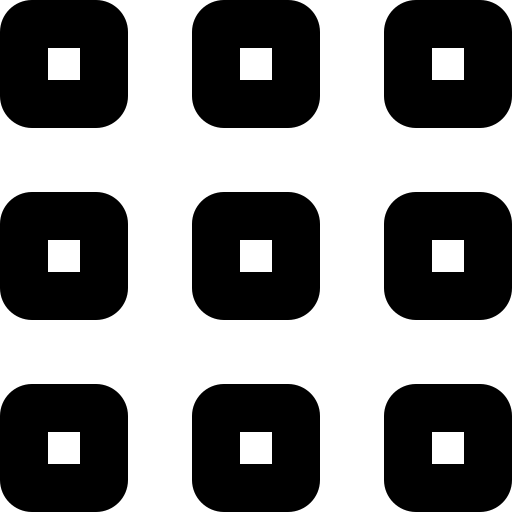
\includegraphics{figures/grid.pdf}

        The poset \verb|Grid(2,[1,1])|.
\end{center}


}\endlist}

\textbf{\hypertarget{Intervals}{\texttt{def Intervals(P)}}}
\addcontentsline{toc}{subsection}{\protect\hyperlink{Intervals}{Intervals}}
{\list{}{\leftmargin 0.5cm}\item{
Returns the lattice of intervals of a given poset (including the empty interval).

\begin{center}
        \includegraphics{figures/interval.pdf}

        The poset \verb|Intervals(Boolean(2))|.
\end{center}

When generating a Hasse diagram with \verb|latex()| use
the prefix \verb|int_| to control options for the node diagrams.


}\endlist}

\textbf{\hypertarget{KleinBottle}{\texttt{def KleinBottle()}}}
\addcontentsline{toc}{subsection}{\protect\hyperlink{KleinBottle}{KleinBottle}}
{\list{}{\leftmargin 0.5cm}\item{
Returns the face poset of a cubical complex homeomorphic to the Klein Bottle.

Pseudonym for \verb|GluedCube([-1,1])|.

}\endlist}

\textbf{\hypertarget{LatticeOfFlats}{\texttt{def LatticeOfFlats(data,as\_genlatt=False)}}}
\addcontentsline{toc}{subsection}{\protect\hyperlink{LatticeOfFlats}{LatticeOfFlats}}
{\list{}{\leftmargin 0.5cm}\item{
Returns the lattice of flats given either a list of edges of a graph or the rank function of a (poly)matroid.

When the input represents a graph it should be in the format \verb|[[i_1,j_1],...,[i_n,j_n]]|
where the pair \verb|[i_k,j_k]| represents an edge between \verb|i_k| and \verb|j_k| in the graph.

When the input represents a (poly)matroid the input should be a list of the ranks of
sets ordered reverse lexicographically (i.e. binary order). For example, if f is the
rank function of a (poly)matroid with ground set size 3 the input should be
        \[
        \verb|[f({}),f({1}),f({2}),f({1,2}),f({3}),f({1,3}),f({2,3}),f({1,2,3})]|.
        \]

When \verb|as_genlatt| is \verb|True| the return value is an instance
of \hyperlink{Genlatt}{\texttt{Genlatt}} with generating set the closures of singletons.

This function may return a poset that isn't a lattice if
the input function isn't submodular or a preorder that isn't a poset if the input
is not order-preserving.

\begin{center}
        \includegraphics{figures/lof_triangle.pdf}

        The poset \verb|LatticeOfFlats([[1,2],[2,3],[3,1]])|.
\end{center}

\begin{center}
        \includegraphics{figures/lof_poly.pdf}

        The poset \verb|LatticeOfFlats([0,1,2,2,1,3,3,3])|.
\end{center}


}\endlist}

\textbf{\hypertarget{MinorPoset}{\texttt{def MinorPoset(L,genL=None, weak=False)}}}
\addcontentsline{toc}{subsection}{\protect\hyperlink{MinorPoset}{MinorPoset}}
{\list{}{\leftmargin 0.5cm}\item{
Returns the minor poset given a lattice \verb|L| and a list of generators \verb|genL|, or a list of edges specifying a graph.

The join irreducibles are automatically added to \verb|genL|. If \verb|genL| is not provided the generating set will be only the
join irreducibles.

If \verb|L| is an instance of the \hyperlink{Poset}{\texttt{Poset}} class then it
is assumed to be a lattice, an instance of \hyperlink{Genlatt}{\texttt{Genlatt}} is
created from \verb|L| and \verb|genL| and the minor poset of
the encoded {\genlatt} is returned. In this case the returned
poset when plotted with \hyperlink{HasseDiagram.latex}{\texttt{Poset.latex}} has elements
represented as {\genlatts}.

If \verb|L| is not an instance of the \hyperlink{Poset}{\texttt{Poset}} class
it should be an iterable of length 2 iterables that
specify edges of a graph. For example, \verb|L=[[1,2],[2,3],[3,1]]|
specifies the 3-cycle graph. The minor poset of the graph
is returned. In this case when plotting the returned poset
with \hyperlink{HasseDiagram.latex}{\texttt{Poset.latex}} the elements are represented as graphs.
Furthermore, there are a few additional options you can use
to control the presentation of the graphs in the Hasse
diagram:
\begin{itemize}
        \item[]{\verb|G_scale| -- Scale of the graph, default is 1.}
        \item[]{\verb|G_pt_size| -- size in points to use for the
        vertices, default is 2.}
        \item[]{\verb|G_node_options| -- Options to place on nodes in the graph, default is \verb|''|.}
        \item[]{\verb|G_node_sep| -- String used to separate names of vertices in the vertex names for minors, default is \verb|'/'|.}
        \item[]{\verb|G_label_dist| -- Distance of vertex to
                its label, default is \verb|1/4|.}
        \item[]{\verb|G_label_scale| -- Scale factor for the
                vertex labels, default is 1.}
\end{itemize}

If \verb|weak| is \verb|True| then the weak minor poset is
returned. Briefly, this poset does not have relations
$(K,H)\le(M,I)$ when some generator $g$ was deleted to form
$(M,I)$ and $g\le\zerohat_K$.

For more info on minor posets see \cite{gustafson-23}.


\begin{center}
        \includegraphics[width=0.4\textwidth]{figures/M_triangle.pdf}

        The poset \verb|MinorPoset([[1,2],[2,3],[3,1]])|.
\end{center}

\begin{center}

        \includegraphics[width=0.4\textwidth]{figures/M_lof_triangle.pdf}
        \hspace{0.5in}
        \includegraphics[width=0.4\textwidth]{figures/M_lof_triangle_weak.pdf}

        On the left the poset \verb|MinorPoset(LatticeOfFlats([[1,2],[2,3],[3,1]]))| and on the right
        the poset \verb|MinorPoset(LatticeOfFlats([[1,2],[2,3],[3,1]]),weak=True)|.
\end{center}

\begin{center}
        \includegraphics[width=0.4\textwidth]{figures/M_lof_poly.pdf}
        \hspace{0.5in}
        \includegraphics[width=0.4\textwidth]{figures/M_lof_poly_weak.pdf}

        On the left the poset \verb|MinorPoset(LatticeOfFlats([0,1,2,2,1,3,3,3]))| and on the right the poset \verb|MinorPoset(LatticeOfFlats([0,1,2,2,1,3,3,3]), weak=True)|.
\end{center}

\begin{center}
        \includegraphics[width=0.4\textwidth]{figures/M_B_2.pdf}
        \hspace{0.5in}
        \includegraphics[width=0.4\textwidth]{figures/M_B_2_weak.pdf}

        On the right the poset \verb|MinorPoset(LatticeOfFlats(Boolean(2),Boolean(2)[1:4]))| and on the left
        the poset \verb|MinorPoset(LatticeOfFlats(Boolean(2),Boolean(2)[1:4]),weak=True)|.
\end{center}


}\endlist}

\textbf{\hypertarget{NoncrossingPartitionLattice}{\texttt{def NoncrossingPartitionLattice(n=3)}}}
\addcontentsline{toc}{subsection}{\protect\hyperlink{NoncrossingPartitionLattice}{NoncrossingPartitionLattice}}
{\list{}{\leftmargin 0.5cm}\item{
Returns the lattice of noncrossing partitions of $1,\dots,n$ ordered by refinement.

\begin{center}
        \includegraphics{figures/NC.pdf}

        The noncrossing partition lattice $\text{NC}_4$.
\end{center}


}\endlist}

\textbf{\hypertarget{PartitionLattice}{\texttt{def PartitionLattice(n=3)}}}
\addcontentsline{toc}{subsection}{\protect\hyperlink{PartitionLattice}{PartitionLattice}}
{\list{}{\leftmargin 0.5cm}\item{
Returns the lattice of partitions of a $1,\dots,n$ ordered by refinement.

\begin{center}
        \includegraphics{figures/Pi.pdf}

        The partition lattice $\Pi_4$.
\end{center}


}\endlist}

\textbf{\hypertarget{Polygon}{\texttt{def Polygon(n)}}}
\addcontentsline{toc}{subsection}{\protect\hyperlink{Polygon}{Polygon}}
{\list{}{\leftmargin 0.5cm}\item{
Returns the face lattice of the $n$-gon.

\begin{center}
        \includegraphics{figures/polygon_4.pdf}

        The poset \verb|Polygon(4)|.
\end{center}


}\endlist}

\textbf{\hypertarget{ProjectiveSpace}{\texttt{def ProjectiveSpace(n=2)}}}
\addcontentsline{toc}{subsection}{\protect\hyperlink{ProjectiveSpace}{ProjectiveSpace}}
{\list{}{\leftmargin 0.5cm}\item{
Returns the face poset of a Cubical complex homeomorphic to projective space of dimension $n$.

Pseudonym for \verb|GluedCube([-1,...,-1])|.

\begin{center}
        \includegraphics{figures/projectiveSpace.pdf}

        The poset \verb|ProjectiveSpace(2)|.
\end{center}


}\endlist}

\textbf{\hypertarget{Root}{\texttt{def Root(n=3)}}}
\addcontentsline{toc}{subsection}{\protect\hyperlink{Root}{Root}}
{\list{}{\leftmargin 0.5cm}\item{
Returns the type $A_{n+1}$ root poset.

\begin{center}
        \includegraphics{figures/root_3.pdf}

        The poset \verb|Root(3)|.
\end{center}


}\endlist}

\textbf{\hypertarget{Simplex}{\texttt{def Simplex(n)}}}
\addcontentsline{toc}{subsection}{\protect\hyperlink{Simplex}{Simplex}}
{\list{}{\leftmargin 0.5cm}\item{
Returns \hyperlink{Boolean}{\texttt{Boolean}}\verb|(n+1)| the face lattice of the $n$-dimensional simplex.

}\endlist}

\textbf{\hypertarget{Torus}{\texttt{def Torus(n=2, m=2)}}}
\addcontentsline{toc}{subsection}{\protect\hyperlink{Torus}{Torus}}
{\list{}{\leftmargin 0.5cm}\item{
Returns the face poset of a cubical complex homeomorphic to the $n$-dimensional Torus.

This poset is isomorphic to the Cartesian product of $n$ copies of $P_m$ with minimum and maximum adjoined
where $P_m$ is the face lattice of an $m$-gon with its minimum and maximum removed.

Let~$\ell_m$ be the $m$th letter of the alphabet.
When $m\le 26$ the set is $\{0,1,\dots,m-1,A,B,\dots,\ell_m\}^n$ and otherwise is $\{0,\dots,m-1,*0,\dots*[m-1]\}^n$.
The order relation is
componentwise where $0<A,\ell_m\ 1<A,B\ \dots\ m-1<\ell_{m-1},\ell_m$  for $m\le26$, and $0<*1,*2\ \dots\  m-1<*[m-1],*0$ for $m>26$.

\begin{center}
        \includegraphics{figures/torus.pdf}

        The poset \verb|Torus(2,2)|.
\end{center}


}\endlist}

\textbf{\hypertarget{Uncrossing}{\texttt{def Uncrossing(t, upper=False, weak=False, E\_only=False, zerohat=True)}}}
\addcontentsline{toc}{subsection}{\protect\hyperlink{Uncrossing}{Uncrossing}}
{\list{}{\leftmargin 0.5cm}\item{
Returns either a lower interval $[\widehat{0},t]$ or the upper interval $[t,\widehat{1}]$ in the uncrossing poset.

The parameter \verb|t| should be either a pairing encoded as a list \verb|[s_1,t_1,...,s_n,t_n]| where
\verb|s_i| is paired to \verb|t_i| or an integer greater than 1. If t is an integer the entire uncrossing
poset of rank $\binom{t}{2}+1$ is returned.

Covers in the uncrossing poset are of the form $\sigma<\tau$
where $\sigma$ is obtained from $\tau$ by swapping points
$i$ and $j$ to remove a crossing.
If \verb|weak| is \verb|True| then the weak subposet
is returned that has cover relations
$\sigma<\tau$ when $\sigma$ is
obtained from $\tau$ by removing a single crossing
via swapping two adjacent points. If \verb|E_only| is
\verb|True| only swaps $(i,j)$ such that the pairing
$\tau$ satisfies $\tau(i)<i$ and $\tau(j)<j$ are used.
These two flags are provided
because this function acts as a backend to \hyperlink{Bruhat}{\texttt{Bruhat}}.
Calling \verb|Uncrossing(n,E_only=True)| constructs
the Bruhat order on $\mathfrak{S_n}$ and adding
\verb|weak=True| constructs the weak order on $\mathfrak{S}_n$.

If \verb|zerohat| is \verb|False| then no minimum is adjoined.

Raises a \verb|ValueError| when \verb|t| is an integer less than 2.

For more info on the uncrossing poset see \cite{lam-15}.

\begin{center}
        \includegraphics{figures/uc.pdf}

        The poset \verb|Uncrossing(3)==Uncrossing([1,4,2,5,3,6])|.
\end{center}


}\endlist}

\textbf{\hypertarget{UniformMatroid}{\texttt{def UniformMatroid(n=3,r=3,q=1)}}}
\addcontentsline{toc}{subsection}{\protect\hyperlink{UniformMatroid}{UniformMatroid}}
{\list{}{\leftmargin 0.5cm}\item{
Returns the lattice of flats of the uniform ($q$-)matroid of rank $r$ on $n$ elements.

Currently only implemented for \verb|q=1| or a prime. Raises an instance of \verb|NotImplementedError| if \verb|q| is neither 1 nor prime.

\begin{center}
        \includegraphics{figures/unif.pdf}

        The poset \verb|UniformMatroid(4,3)|.
\end{center}

\begin{center}
        \includegraphics{figures/qunif.pdf}

        The poset \verb|UniformMatroid(4,3,2)|.
\end{center}


}\endlist}

\section{Polynomial}
\label{Polynomial}

\textbf{\hypertarget{Polynomial}{\Large \texttt{class Polynomial}}}

{\list{}{\leftmargin 0.5cm}\item{
A class encoding polynomials in noncommutative variables (used by the \hyperlink{Poset}{\texttt{Poset}} class to compute the \cv\dv-index).

This class is basically a wrapper around a dictionary representation for polynomials (e.g. $3\av\bv+2\bv\bv$ is encoded as \verb|{'ab':3, 'bb':2}|).
The class provides methods for basic arithmetic with polynomials, to substitute a polynomial
for a variable in another polynomial and to convert \av\bv-polynomials to \cv\dv-polynomials (when possible) and vice versa. You can also get and set
coefficients as if a polynomial were a dictionary.

}\endlist}


\begin{child}
\textbf{\hypertarget{Polynomial.__add__}{\texttt{def \_\_add\_\_(*args)}}}
\addcontentsline{toc}{subsection}{\protect\hyperlink{Polynomial.__add__}{\_\_add\_\_}}
{\list{}{\leftmargin 0.5cm}\item{
Polynomial addition.

Raises \verb|NotImplementedError| if the coefficients can't be aded.
}\endlist}

\textbf{\hypertarget{Polynomial.__bool__}{\texttt{def \_\_bool\_\_(this)}}}
\addcontentsline{toc}{subsection}{\protect\hyperlink{Polynomial.__bool__}{\_\_bool\_\_}}
{\list{}{\leftmargin 0.5cm}\item{}\endlist}

\textbf{\hypertarget{Polynomial.__eq__}{\texttt{def \_\_eq\_\_(this,that)}}}
\addcontentsline{toc}{subsection}{\protect\hyperlink{Polynomial.__eq__}{\_\_eq\_\_}}
{\list{}{\leftmargin 0.5cm}\item{}\endlist}

\textbf{\hypertarget{Polynomial.__floordiv__}{\texttt{def \_\_floordiv\_\_(this,that)}}}
\addcontentsline{toc}{subsection}{\protect\hyperlink{Polynomial.__floordiv__}{\_\_floordiv\_\_}}
{\list{}{\leftmargin 0.5cm}\item{}\endlist}

\textbf{\hypertarget{Polynomial.__ge__}{\texttt{def \_\_ge\_\_(this, that)}}}
\addcontentsline{toc}{subsection}{\protect\hyperlink{Polynomial.__ge__}{\_\_ge\_\_}}
{\list{}{\leftmargin 0.5cm}\item{
Returns \verb|True| if \verb|this| is coefficientwise
greater than or equal
to \verb|that|.
}\endlist}

\textbf{\hypertarget{Polynomial.__getitem__}{\texttt{def \_\_getitem\_\_(this,i)}}}
\addcontentsline{toc}{subsection}{\protect\hyperlink{Polynomial.__getitem__}{\_\_getitem\_\_}}
{\list{}{\leftmargin 0.5cm}\item{}\endlist}

\textbf{\hypertarget{Polynomial.__gt__}{\texttt{def \_\_gt\_\_(this, that)}}}
\addcontentsline{toc}{subsection}{\protect\hyperlink{Polynomial.__gt__}{\_\_gt\_\_}}
{\list{}{\leftmargin 0.5cm}\item{
Returns \verb|True| if \verb|this| is greater than or equal
to \verb|that| coefficientwise and \verb|this| is not equal
to \verb|that|.
}\endlist}

\textbf{\hypertarget{Polynomial.__init__}{\texttt{def \_\_init\_\_(this, data=None)}}}
\addcontentsline{toc}{subsection}{\protect\hyperlink{Polynomial.__init__}{\_\_init\_\_}}
{\list{}{\leftmargin 0.5cm}\item{
Returns a \hyperlink{Polynomial}{\texttt{Polynomial}} given a dictionary.

The keys in \verb|data| are the monomials, encoded as
strings, and the values are the coefficients.
Coefficients can be any class that supports addition and
multiplication and such that comparing to 0 returns a boolean.

If \verb|data| is \verb|None| or an empty dictionary then 
the zero polynomial is returned.
}\endlist}

\textbf{\hypertarget{Polynomial.__iter__}{\texttt{def \_\_iter\_\_(this)}}}
\addcontentsline{toc}{subsection}{\protect\hyperlink{Polynomial.__iter__}{\_\_iter\_\_}}
{\list{}{\leftmargin 0.5cm}\item{}\endlist}

\textbf{\hypertarget{Polynomial.__le__}{\texttt{def \_\_le\_\_(this, that)}}}
\addcontentsline{toc}{subsection}{\protect\hyperlink{Polynomial.__le__}{\_\_le\_\_}}
{\list{}{\leftmargin 0.5cm}\item{
Returns \verb|True| if \verb|this| is coefficientwise less or
equal to \verb|that|.
}\endlist}

\textbf{\hypertarget{Polynomial.__len__}{\texttt{def \_\_len\_\_(this)}}}
\addcontentsline{toc}{subsection}{\protect\hyperlink{Polynomial.__len__}{\_\_len\_\_}}
{\list{}{\leftmargin 0.5cm}\item{Returns the number of coefficients.}\endlist}

\textbf{\hypertarget{Polynomial.__lt__}{\texttt{def \_\_lt\_\_(this, that)}}}
\addcontentsline{toc}{subsection}{\protect\hyperlink{Polynomial.__lt__}{\_\_lt\_\_}}
{\list{}{\leftmargin 0.5cm}\item{
Returns \verb|True| if \verb|this| is coefficientwise less or
equal to \verb|that| and \verb|this| and \verb|that| or not equal.
}\endlist}

\textbf{\hypertarget{Polynomial.__mod__}{\texttt{def \_\_mod\_\_(this,that)}}}
\addcontentsline{toc}{subsection}{\protect\hyperlink{Polynomial.__mod__}{\_\_mod\_\_}}
{\list{}{\leftmargin 0.5cm}\item{}\endlist}

\textbf{\hypertarget{Polynomial.__mul__}{\texttt{def \_\_mul\_\_(*args)}}}
\addcontentsline{toc}{subsection}{\protect\hyperlink{Polynomial.__mul__}{\_\_mul\_\_}}
{\list{}{\leftmargin 0.5cm}\item{
Noncommutative polynomial multiplication.
}\endlist}

\textbf{\hypertarget{Polynomial.__neg__}{\texttt{def \_\_neg\_\_(this)}}}
\addcontentsline{toc}{subsection}{\protect\hyperlink{Polynomial.__neg__}{\_\_neg\_\_}}
{\list{}{\leftmargin 0.5cm}\item{}\endlist}

\textbf{\hypertarget{Polynomial.__pow__}{\texttt{def \_\_pow\_\_(this,x)}}}
\addcontentsline{toc}{subsection}{\protect\hyperlink{Polynomial.__pow__}{\_\_pow\_\_}}
{\list{}{\leftmargin 0.5cm}\item{
Polynomial exponentiation by non-negative integers.

Raises \verb|NotImplementedError| if either \verb|x| is
not an integer or \verb|x<0|.
}\endlist}

\textbf{\hypertarget{Polynomial.__add__}{\texttt{def \_\_add\_\_(*args)}}}
\addcontentsline{toc}{subsection}{\protect\hyperlink{Polynomial.__add__}{\_\_add\_\_}}
{\list{}{\leftmargin 0.5cm}\item{
Polynomial addition.

Raises \verb|NotImplementedError| if the coefficients can't be aded.
}\endlist}

\textbf{\hypertarget{Polynomial.__repr__}{\texttt{def \_\_repr\_\_(this)}}}
\addcontentsline{toc}{subsection}{\protect\hyperlink{Polynomial.__repr__}{\_\_repr\_\_}}
{\list{}{\leftmargin 0.5cm}\item{}\endlist}

\textbf{\hypertarget{Polynomial.__mul__}{\texttt{def \_\_mul\_\_(*args)}}}
\addcontentsline{toc}{subsection}{\protect\hyperlink{Polynomial.__mul__}{\_\_mul\_\_}}
{\list{}{\leftmargin 0.5cm}\item{
Noncommutative polynomial multiplication.
}\endlist}

\textbf{\hypertarget{Polynomial.__setitem__}{\texttt{def \_\_setitem\_\_(this,i,value)}}}
\addcontentsline{toc}{subsection}{\protect\hyperlink{Polynomial.__setitem__}{\_\_setitem\_\_}}
{\list{}{\leftmargin 0.5cm}\item{}\endlist}

\textbf{\hypertarget{Polynomial.__str__}{\texttt{def \_\_str\_\_(this)}}}
\addcontentsline{toc}{subsection}{\protect\hyperlink{Polynomial.__str__}{\_\_str\_\_}}
{\list{}{\leftmargin 0.5cm}\item{}\endlist}

\textbf{\hypertarget{Polynomial.__sub__}{\texttt{def \_\_sub\_\_(this, that)}}}
\addcontentsline{toc}{subsection}{\protect\hyperlink{Polynomial.__sub__}{\_\_sub\_\_}}
{\list{}{\leftmargin 0.5cm}\item{Polynomial subtraction}\endlist}

\textbf{\hypertarget{Polynomial.__truediv__}{\texttt{def \_\_truediv\_\_(this,that)}}}
\addcontentsline{toc}{subsection}{\protect\hyperlink{Polynomial.__truediv__}{\_\_truediv\_\_}}
{\list{}{\leftmargin 0.5cm}\item{}\endlist}

\textbf{\hypertarget{Polynomial._coeff_str}{\texttt{def \_coeff\_str(c)}}}
\addcontentsline{toc}{subsection}{\protect\hyperlink{Polynomial._coeff_str}{\_coeff\_str}}
{\list{}{\leftmargin 0.5cm}\item{}\endlist}

\textbf{\hypertarget{Polynomial._monom_str}{\texttt{def \_monom\_str(m)}}}
\addcontentsline{toc}{subsection}{\protect\hyperlink{Polynomial._monom_str}{\_monom\_str}}
{\list{}{\leftmargin 0.5cm}\item{}\endlist}

\textbf{\hypertarget{Polynomial._poly_add_prepoly}{\texttt{def \_poly\_add\_prepoly(p, q)}}}
\addcontentsline{toc}{subsection}{\protect\hyperlink{Polynomial._poly_add_prepoly}{\_poly\_add\_prepoly}}
{\list{}{\leftmargin 0.5cm}\item{Internal backend for \verb|__add__|.}\endlist}

\textbf{\hypertarget{Polynomial._prepoly_mul_poly}{\texttt{def \_prepoly\_mul\_poly(q, p)}}}
\addcontentsline{toc}{subsection}{\protect\hyperlink{Polynomial._prepoly_mul_poly}{\_prepoly\_mul\_poly}}
{\list{}{\leftmargin 0.5cm}\item{Internal backend for \verb|__mul__|.}\endlist}

\textbf{\hypertarget{Polynomial.abToCd}{\texttt{def abToCd(this)}}}
\addcontentsline{toc}{subsection}{\protect\hyperlink{Polynomial.abToCd}{abToCd}}
{\list{}{\leftmargin 0.5cm}\item{
Given an \av\bv-polynomial returns the corresponding \cv\dv-polynomial if possible and the given polynomial if not.
}\endlist}

\textbf{\hypertarget{Polynomial.cdToAb}{\texttt{def cdToAb(this)}}}
\addcontentsline{toc}{subsection}{\protect\hyperlink{Polynomial.cdToAb}{cdToAb}}
{\list{}{\leftmargin 0.5cm}\item{
Given a \cv\dv-polynomial returns the corresponding \av\bv-polynomial.
}\endlist}

\textbf{\hypertarget{Polynomial.strip}{\texttt{def strip(this)}}}
\addcontentsline{toc}{subsection}{\protect\hyperlink{Polynomial.strip}{strip}}
{\list{}{\leftmargin 0.5cm}\item{
Removes any zero terms from a polynomial in place and returns it.
}\endlist}

\textbf{\hypertarget{Polynomial.sub}{\texttt{def sub(this, poly, monom)}}}
\addcontentsline{toc}{subsection}{\protect\hyperlink{Polynomial.sub}{sub}}
{\list{}{\leftmargin 0.5cm}\item{
Returns the polynomial obtained by substituting the polynomial \verb|poly| for the monomial \verb|m| (given as a string) in \verb|this|.
}\endlist}

\end{child}














\section{TriangularArray}
\label{TriangularArray}

\textbf{\hypertarget{TriangularArray}{\Large \texttt{class TriangularArray}}}

{\list{}{\leftmargin 0.5cm}\item{
A class encoding a triangular array.

This class is used to encode the zeta function of a poset.

Constructor arguments:
\begin{itemize}
        \item[]{\verb|data| -- An iterable specifying the entries in the upper diagonal; may be either a flat list or an iterable of iterables.}
        \item[]{\verb|flat| -- Whether the data is in flat form or not.}
        \end{itemize}
Constructor raises \verb|ValueError| if the number of entries of \verb|data| is not a triangle number.


}\endlist}


\begin{child}
\textbf{\hypertarget{TriangularArray.__eq__}{\texttt{def \_\_eq\_\_(this,that)}}}
\addcontentsline{toc}{subsection}{\protect\hyperlink{TriangularArray.__eq__}{\_\_eq\_\_}}
{\list{}{\leftmargin 0.5cm}\item{}\endlist}

\textbf{\hypertarget{TriangularArray.__getitem__}{\texttt{def \_\_getitem\_\_(this, x)}}}
\addcontentsline{toc}{subsection}{\protect\hyperlink{TriangularArray.__getitem__}{\_\_getitem\_\_}}
{\list{}{\leftmargin 0.5cm}\item{
Zero based indexing $(i,j)$  gives the element in row $i$ and column $j$.

The argument \verb|x| must be a tuple of integers such that $0\le x_0\le x_1< n$ where $n$ is the size of the triangular array.
}\endlist}

\textbf{\hypertarget{TriangularArray.__init__}{\texttt{def \_\_init\_\_(this, data, flat=True)}}}
\addcontentsline{toc}{subsection}{\protect\hyperlink{TriangularArray.__init__}{\_\_init\_\_}}
{\list{}{\leftmargin 0.5cm}\item{}\endlist}

\textbf{\hypertarget{TriangularArray.__repr__}{\texttt{def \_\_repr\_\_(this)}}}
\addcontentsline{toc}{subsection}{\protect\hyperlink{TriangularArray.__repr__}{\_\_repr\_\_}}
{\list{}{\leftmargin 0.5cm}\item{}\endlist}

\textbf{\hypertarget{TriangularArray.__setitem__}{\texttt{def \_\_setitem\_\_(this, idx, x)}}}
\addcontentsline{toc}{subsection}{\protect\hyperlink{TriangularArray.__setitem__}{\_\_setitem\_\_}}
{\list{}{\leftmargin 0.5cm}\item{}\endlist}

\textbf{\hypertarget{TriangularArray.__str__}{\texttt{def \_\_str\_\_(this)}}}
\addcontentsline{toc}{subsection}{\protect\hyperlink{TriangularArray.__str__}{\_\_str\_\_}}
{\list{}{\leftmargin 0.5cm}\item{}\endlist}

\textbf{\hypertarget{TriangularArray.col}{\texttt{def col(this, j)}}}
\addcontentsline{toc}{subsection}{\protect\hyperlink{TriangularArray.col}{col}}
{\list{}{\leftmargin 0.5cm}\item{
Generator for the $i$th column.
}\endlist}

\textbf{\hypertarget{TriangularArray.inverse}{\texttt{def inverse(this)}}}
\addcontentsline{toc}{subsection}{\protect\hyperlink{TriangularArray.inverse}{inverse}}
{\list{}{\leftmargin 0.5cm}\item{
Returns the inverse of the triangular array considered as an upper triangular matrix.

Raises \verb|ZeroDivisionError| if a diagonal entry of the array is zero.
}\endlist}

\textbf{\hypertarget{TriangularArray.revtranspose}{\texttt{def revtranspose(this)}}}
\addcontentsline{toc}{subsection}{\protect\hyperlink{TriangularArray.revtranspose}{revtranspose}}
{\list{}{\leftmargin 0.5cm}\item{
Returns a new instance of \hyperlink{TriangularArray}{\texttt{TriangularArray}} obtained by transposing and reversing all columns and rows.
}\endlist}

\textbf{\hypertarget{TriangularArray.row}{\texttt{def row(this, i)}}}
\addcontentsline{toc}{subsection}{\protect\hyperlink{TriangularArray.row}{row}}
{\list{}{\leftmargin 0.5cm}\item{
Returns the $i$th row as a list.
}\endlist}

\textbf{\hypertarget{TriangularArray.subarray}{\texttt{def subarray(this, S)}}}
\addcontentsline{toc}{subsection}{\protect\hyperlink{TriangularArray.subarray}{subarray}}
{\list{}{\leftmargin 0.5cm}\item{
Returns a sub-triangular array by selecting the rows and columns indexed by \verb|S|.
}\endlist}

\end{child}



\section{ZetaHasseDiagram}
\label{ZetaHasseDiagram}

\textbf{\hypertarget{ZetaHasseDiagram}{\Large \texttt{class ZetaHasseDiagram(SubposetsHasseDiagram)}}}

{\list{}{\leftmargin 0.5cm}\item{
Class to draw the Hasse diagram of a poset as principal filters (or ideals) labeled by the zeta function values.

This is a convenience class that merely passes appropriate options to \hyperlink{SubposetsHasseDiagram}{\texttt{SubposetsHasseDiagram}}.
When \verb|latex| is called this class produces latex code for the Hasse diagram of the given
poset $P$ with each element $p$ as the principal filter $\{q\in P:q\ge p\}$ (or optionally the principal
ideal) with each element $q$ in the filter labeled by $\zeta(p,q)$.

This class is intended for representing quasigraded posets, those with a zeta function taking values
other than 0 and 1.

Constructor arguments:
\begin{itemize}
        \item[]{\verb|filters| -- Whether to represent elements by the associated principal
                filter or alternatively as ideals. The default value is \verb|True| which
                will use filters.
                }
        \item[]{\verb|keep_ranks| -- Whether to use the same rank values for elements in
                the filters/ideals drawn as in the given poset. If this argument is \verb|False|
                then a new poset is created with rank function the standard length function
                as returned by \hyperlink{Poset.make_ranks}{\texttt{Poset.make\_ranks}}.
                }
\end{itemize}


See \hyperlink{SubposetsHasseDiagram}{\texttt{SubposetsHasseDiagram}} for details on other arguments. Note, the argument \verb|prefix| to
\hyperlink{SubposetsHasseDiagram}{\texttt{SubposetsHasseDiagram}} defaults to \verb|'V'|.

Note, if \verb|V_width| (or \verb|V_height|) is not provided (assuming
the default value \verb|'V'| for \verb|prefix|) it is set to one fifth
of \verb|width| (or \verb|height|).
If \verb|V_nodescale| is not provided it is set to \verb|0.5|.


}\endlist}


\begin{child}
\textbf{\hypertarget{ZetaHasseDiagram.__init__}{\texttt{def \_\_init\_\_(this, P, filters=True, prefix='V', keep\_ranks=True, func\_args=None,}}}\\
\textbf{\texttt{**kwargs)}}
\\
\addcontentsline{toc}{subsection}{\protect\hyperlink{ZetaHasseDiagram.__init__}{\_\_init\_\_}}
{\list{}{\leftmargin 0.5cm}\item{
See \hyperlink{ZetaHasseDiagram}{\texttt{ZetaHasseDiagram}}.
}\endlist}

\end{child}





\bibliography{bib}{}
\bibliographystyle{plain}
\end{document}